% /*
%  * ----------------------------------------------------------------------------
%  * "THE BEER-WARE LICENSE" (Revision 42):
%  * <michi.wieland@hotmail.com> wrote this file. As long as you retain this notice you
%  * can do whatever you want with this stuff. If we meet some day, and you think
%  * this stuff is worth it, you can buy me a beer in return. Michael Wieland
%  * ----------------------------------------------------------------------------
%  */

\documentclass[
a4paper,
oneside,
10pt,
fleqn,
headsepline,
toc=listofnumbered, 
bibliography=totocnumbered]{scrartcl}

% deutsche Trennmuster etc.
\usepackage[T1]{fontenc}
\usepackage[utf8]{inputenc}
\usepackage[english, ngerman]{babel} % \selectlanguage{english} if  needed
\usepackage{lmodern} % use modern latin fonts

% Custom commands
\newcommand{\AUTHOR}{Michael Wieland}
\newcommand{\INSTITUTE}{Hochschule für Technik Rapperswil}
\newcommand{\GITHUB}{https://github.com/michiwieland/hsr-zusammenfassungen}
\newcommand{\LICENSEURL}{https://en.wikipedia.org/wiki/Beerware}
\newcommand{\LICENSE}{
"THE BEER-WARE LICENSE" (Revision 42):
<michi.wieland@hotmail.com> wrote this file. As long as you retain this notice you
can do whatever you want with this stuff. If we meet some day, and you think
this stuff is worth it, you can buy me a beer in return. Michael Wieland	
}

% Jede Überschrift 1 auf neuer Seite
\let\stdsection\section
\renewcommand\section{\clearpage\stdsection}

% Multiple Authors
\usepackage{authblk}

% Include external pdf
\usepackage{pdfpages}

% Layout / Seitenränder
\usepackage{geometry}

% Inhaltsverzeichnis
\usepackage{makeidx} 
\makeindex

\usepackage{url}
\usepackage[pdfborder={0 0 0}]{hyperref}
\usepackage[all]{hypcap}
\usepackage{hyperxmp} % for license metadata

% Glossar und Abkürzungsverzeichnis
\usepackage[acronym,toc,nopostdot]{glossaries}
\glossarystyle{altlist}
\usepackage{xparse}
\DeclareDocumentCommand{\newdualentry}{ O{} O{} m m m m } {
	\newglossaryentry{gls-#3}{
		name={#4 : #5},
		text={#5\glsadd{#3}},
		description={#6},
		#1
	}
	\makeglossaries
	\newacronym[see={[Siehe:]{gls-#3}},#2]{#3}{#4}{#5\glsadd{gls-#3}}
}
\makeglossaries

% Mathematik
\usepackage{amsmath}
\usepackage{amssymb}
\usepackage{amsfonts}
\usepackage{enumitem}

% Images
\usepackage{graphicx}
\graphicspath{{images/}} % default paths

% Boxes
\usepackage{fancybox}

%Tables
\usepackage{tabu}
\usepackage{booktabs} % toprule, midrule, bottomrule
\usepackage{array} % for matrix tables

% Multi Columns
\usepackage{multicol}

% Header and footer
\usepackage{scrlayer-scrpage}
\setkomafont{pagehead}{\normalfont}
\setkomafont{pagefoot}{\normalfont}
\automark*{section}
\clearpairofpagestyles
\ihead{\headmark}
\ohead{\AUTHOR}
\cfoot{\pagemark}

% Pseudocode
\usepackage{algorithmic}
\usepackage[linesnumbered,ruled]{algorithm2e}

% Code Listings
\usepackage{listings}
\usepackage{color}
\usepackage{beramono}

\definecolor{bluekeywords}{rgb}{0,0,1}
\definecolor{greencomments}{rgb}{0,0.5,0}
\definecolor{redstrings}{rgb}{0.64,0.08,0.08}
\definecolor{xmlcomments}{rgb}{0.5,0.5,0.5}
\definecolor{types}{rgb}{0.17,0.57,0.68}

\lstdefinestyle{visual-studio-style}{
	language=[Sharp]C,
	columns=flexible,
	showstringspaces=false,
	basicstyle=\footnotesize\ttfamily, 
	commentstyle=\color{greencomments},
	morekeywords={partial, var, value, get, set},
	keywordstyle=\bfseries\color{bluekeywords},
	stringstyle=\color{redstrings},
	breaklines=true,
	breakatwhitespace=true,
	tabsize=4,
	numbers=left,
	numberstyle=\tiny\color{black},
	frame=lines,
	showspaces=false,
	showtabs=false,
	escapeinside={£}{£},
}

\definecolor{DarkPurple}{rgb}{0.4, 0.1, 0.4}
\definecolor{DarkCyan}{rgb}{0.0, 0.5, 0.4}
\definecolor{LightLime}{rgb}{0.3, 0.5, 0.4}
\definecolor{Blue}{rgb}{0.0, 0.0, 1.0}

\lstdefinestyle{cevelop-style}{
	language=C++,  
	columns=flexible,
	showstringspaces=false,     
	basicstyle=\footnotesize\ttfamily, 
	keywordstyle=\bfseries\color{DarkPurple},
	commentstyle=\color{LightLime},
	stringstyle=\color{Blue}, 
	escapeinside={£}{£}, % latex scope within code      
	breaklines=true,
	breakatwhitespace=true,
	showspaces=false,
	showtabs=false,
	tabsize=4,
	morekeywords={include,ifndef,define},
	numbers=left,
	numberstyle=\tiny\color{black},
	frame=lines,
}

\lstdefinestyle{eclipse-style}{
	language=Java,  
	columns=flexible,
	showstringspaces=false,     
	basicstyle=\footnotesize\ttfamily, 
	keywordstyle=\bfseries\color{DarkPurple},
	commentstyle=\color{LightLime},
	stringstyle=\color{Blue}, 
	escapeinside={£}{£}, % latex scope within code      
	breaklines=true,
	breakatwhitespace=true,
	showspaces=false,
	showtabs=false,
	tabsize=4,
	morekeywords={length},
	numbers=left,
	numberstyle=\tiny\color{black},
	frame=lines,
}
\lstset{style=eclipse-style}



% Theorems \begin{mytheo}{title}{label}
\usepackage{tcolorbox}
\tcbuselibrary{theorems}
\newtcbtheorem[number within=section]{definiton}{Definition}%
{fonttitle=\bfseries}{def}
\newtcbtheorem[number within=section]{remember}{Merke}%
{fonttitle=\bfseries}{rem}
\newtcbtheorem[number within=section]{hint}{Hinweis}%
{fonttitle=\bfseries}{hnt}

% Dokumentinformationen
\newcommand{\SUBJECT}{Zusammenfassung}
\newcommand{\TITLE}{C++}

\loadglsentries{glossar}

% pdf metadata
\hypersetup{
	pdfauthor={\AUTHOR},
	pdftitle={\SUBJECT \TITLE},
	pdfcopyright={\LICENSE},
	pdflicenseurl={\LICENSEURL}
}

\begin{document}
	
% Front page
\title{\TITLE}
\subject{\SUBJECT}
\author{\AUTHOR}
\affil{\INSTITUTE}
\date{\today}
\maketitle

\vfill

% Participate
\paragraph{Mitmachen} \hfill \\
Falls Du an diesem Dokument mitarbeiten willst, kannst Du das Dokument
auf GitHub unter \url{\GITHUB} forken.

% Licence
\paragraph{Lizenz} \hfill \\
\LICENSE

% Table of contents
\tableofcontents


% Glossar and acronyms (if included \loadglsentries{glossar})
\printglossary[type=\acronymtype]
\printglossary
\glsaddall


\lstset{style=cevelop-style}

\section{Konzepte: Der heilige Gral}
\begin{itemize}
	\item In C++ sind alles standardmässig Wertetypen und werden auf dem Stack alloziert
	\item Klassenmember sind implizit \lstinline|inline| und \lstinline|private|. Bei Structs sind die Member implizit \lstinline|public|.
	\item Der Copy Konstruktor ist implizit verfügbar
	\item Parameter werden standardmässig \textbf{By Value} übergeben. Das beudetet, es wird eine Kopie des Parameters angelegt. Dies ist ein Problem bei grösseren Objekten. Man sollte diese deshalb mit dem \lstinline|&| Operator explizit \textbf{By Reference} übergeben.
	\item Unveränderbare grosse Objekte sollten per \lstinline|const &| (Const Referenz) übergeben werden
	\item Zur Funktionssignatur wird der Name, die Parameter und \lstinline|const| dazugezählt.
	\item '';'' hinter jede Klasse, Struct und Enum
	\item Konstruktoren mit Parameter sollten als \lstinline |explicit| deklariert werden. \\
	\lstinline|explicit MyClass(int a, int b)  : _a{a}, _b{b} {..validate..}|
	\item Variablen initialisieren mit geschweifte Klammern \lstinline|{}| oder \lstinline|=| bei \lstinline|auto| Variablen (Theoretisch geht auch \lstinline|={}|)
	\item Alles was nicht verändert wird oder etwas verändert \lstinline|const| deklarieren.
	\item \lstinline|const| Variablen müssen \textbf{direkt oder im Konstruktor} initialisiert werden.
	\item Nie Referenzen auf lokale Variablen einer Funktion zurückgeben, da der Stack nach dem Funktionsaufruf abgebaut wird.
	\item Es gibt zwei Variaten um auf das \lstinline|this| Objekt zuzugreifen: \lstinline|this->m();| und \lstinline|(*this).m();|
	\item Eine Methode in der Basisklasse kann über eine Typendefinition aufgerufen werden. \\
	\lstinline|using super = std::WHATEVER<T>; super::method();|
	\item Functoren überladen den call Operator: \lstinline|void operator()(int value) {..}|
	\item Bei Template Klassen sollte auf vererbte Member immer über das \lstinline|this| Objekt zugegriffen werden. 
	\item Memberfunktionen die nie benutzt werden, werden bei Template Klasse nie kompiliert.
	\item Mit dem \lstinline|class| Keyword (Scoped) Enum ist der Enum nur innerhalb des Namespaces sichtbar. Ansonsten global.
	\item (std::string = \lstinline|"mystring"s|) $\neq$ \lstinline|"ab"| (char array)
\end{itemize}

\subsection{Vererbung}
\begin{itemize}
	\item Beim \textbf{Aufbau} der Objekte bei der Vererbung: von Base	nach Sub	
	\item Beim \textbf{Abbau} der Objekte bei der Vererbung: von Sub nach	Base.	 
	\item Bei Mehrfachvererbung wird von links nach rechts die Konstruktoren aufgerufen. Bei der Dekonstruktion genau umgekehrt
	\item Bei Mehrfachvererbung wird der Parent bei der Diamanten Form mehrere Male aufgerufen
	\item Vererbung ist bei Klassen standardmässig \lstinline|private|. Möchten man die Membervariablen des Base Klasse nach aussen tragen, muss dies explit angegeben werden. (\lstinline|class MyClass<T> : public Base<T> {..}|)
	\item Bei Structs ist die Vererbung implizit \lstinline|public|
	\item Beim \textbf{Object Slicing} ist der statische und dynamische Typ gleich
\end{itemize}
\paragraph{Konstruktoren}
\begin{itemize}
	\item Der Copy Konstruktor ist ein impliziter, eigenständiger Konstruktur und führt keine anderen Konstruktoren aus.	
	\item Beim Copy Konstruktor gibt es immer Object Slicing. Er ist implizit verfügbar.
	\item Die Konstruktoren werden nicht implizit vererbt
\end{itemize}

\paragraph{Methoden Overloading / Overriding}
\begin{itemize}
	\item Ist der statische Typ nicht mit dem dynamischen Typ identisch, werden die Methoden im Parent gesucht
	\item \lstinline|const| wird zur Signatur gezählt
	\item Sobald eine Methode virtual ist, kommt Dynamic Dispatch zum Zug (Methode des dynamischen Typs wird genommen). Sonst die Methode des statischen Typs.
	\item Bei überdeckten Methoden wird die Methode im statischen Typ ausgegeben.
	\item Ist die Methode im Parent \lstinline|virtual|, sind die Methoden in den Childs \textbf{implizit} \lstinline|virtual|
\end{itemize}

\paragraph{Referenzen}
\begin{itemize}
	\item Bei einer Referenz wird kein neues Objekt erstellt: \\ \textbf{Statischer Typ}: Neuer Typ und \textbf{Dynamischer Typ}: alter Typ. Es wird kein Konstruktor aufgerufen!
	\item Zuweisungen oder übermitteln von Parameter \lstinline|by value| von abgeleiteten Klassen in Variablen vom Typ der Base Klasse resultieren in \textbf{Object Slicing} \\ $\rightarrow$ Nur Base-Class Member Variablen werden behaldent. (\lstinline|MyBase base = subVar;|)	
	\item Bei Referenzen wird kein Destruktor aufgerufen	
\end{itemize}

\paragraph{Häufige Fehler}
\begin{itemize}
	\item Kein	virtueller Dekonstruktor $\rightarrow$ häufig	zur	Folge, dass die Objekte nicht sauber abgeräumt werden können. Dekonstrukoren sollten deshalb virtual sein, wenn eine Methode virtual ist.
	\item Function Hiding: Nicht virtuelle Methoden werden in der Subclass überschrieben.
	\item Member Funktionen, die nichts verändern, sollten const sein.
	\item Mehrfachvererbung 
\end{itemize}

\clearpage

\subsection{Iteratoren}
\begin{itemize}
	\item Der Stern-Operator(*) bindet mehr als	''+1'' (Präzedenz) $\rightarrow$ Char wird ausgelesen und dann +1 gezählt $\rightarrow$ nächster	Buchstabe aus ASCII	
	\item \lstinline|(*it)++| = Wert wird gelesen und inkrementiert
	\item \lstinline|*(it++)| = Inkrementiert den Iterator und greift dann auf das Objekt zu
	\item Geht man mit dem \lstinline|std::advance| Algorithmus über den Bereich des Containers, resultiert \textbf{Undefined behaviour}
	\item Inklusive Leerzeichen: \lstinline|using it = std::istreambuf_iterator<char>;|
	\item Exklusive Leerzeichen: \lstinline|using it = std::istream_iterator<char>;|
	\item Bei \lstinline|rend()| muss \lstinline|--| genommen werden, um nach ''vorne'' zu iterieren
	\item \lstinline|std::advance(it, 2)| verändert das \lstinline|it| Argument. Gibt nichts zurück. 
	\item \lstinline|std::next(it, -2)| verändert das \lstinline|it| Argument nicht. Gibt eine Kopie des Iterators zurück (verschoben um x)
\end{itemize}
\begin{lstlisting}[language=C++]
// replace WHATEVER!
std::WHATEVER::iterator 
std::WHATEVER::const_iterator 
std::WHATEVER::reverse_iterator 
std::WHATEVER::const_reverse_iterator 

rbegin() = --end() 
rend() = --begin()
\end{lstlisting}

\begin{figure}[h]
	\centering
	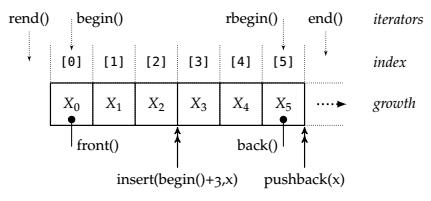
\includegraphics[width=0.7\linewidth]{images/iterator}
	\caption{Iteratoren}
	\label{fig:iterator}
\end{figure}


\clearpage

\subsection{ASCII Tabelle}
A B C D E F G H I J K L M N O P Q R S T U V W X Y Z \\
a b c d e f g h i j k l m n o p q r s t u v w x y z
\begin{figure}[h!]
	\centering
	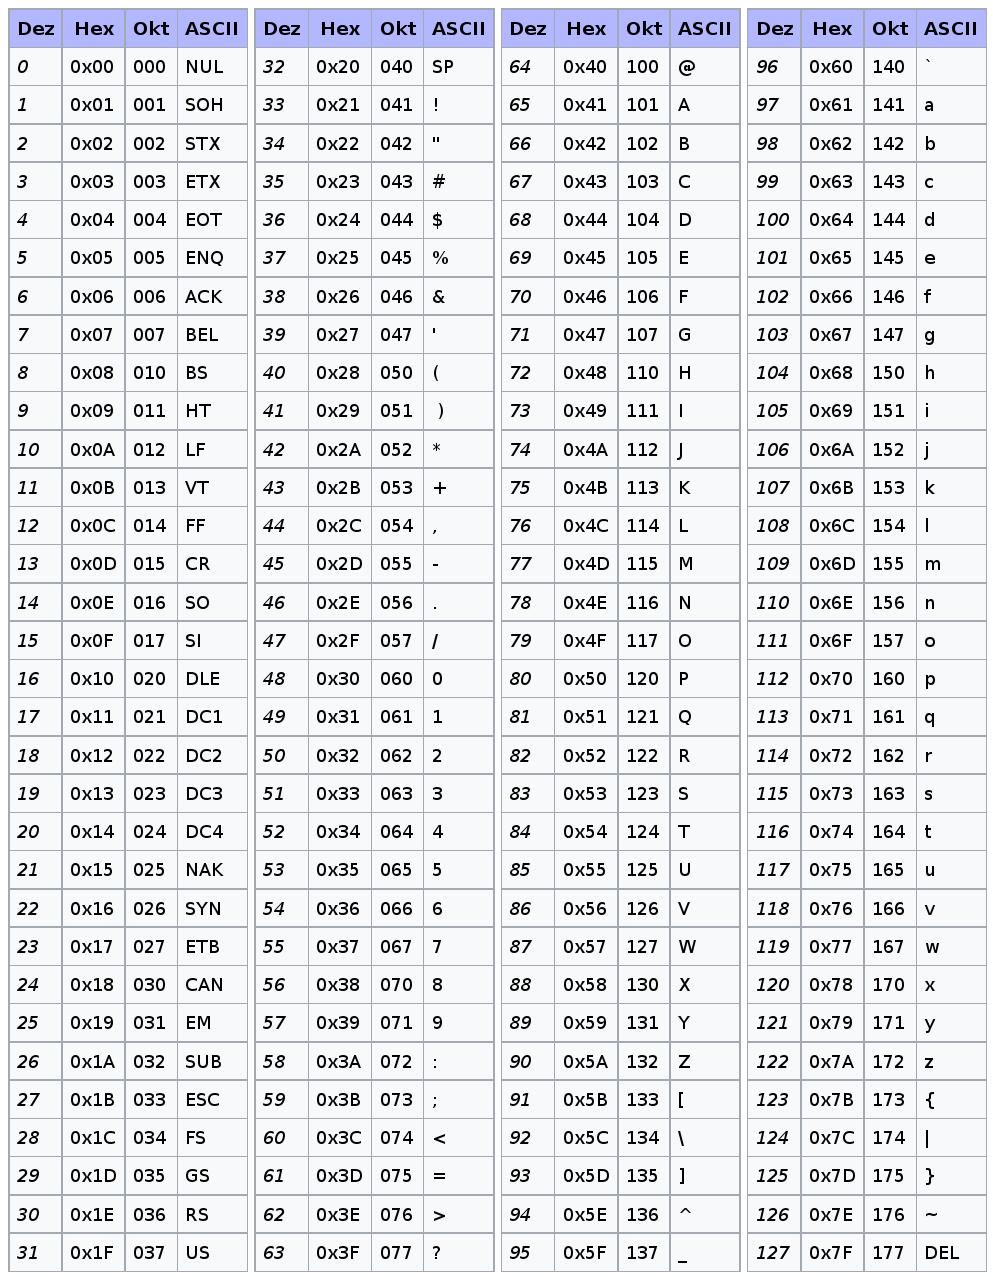
\includegraphics[width=0.9\linewidth]{images/ascii_table}
	\caption{ASCII Tabelle}
	\label{fig:asciitable}
\end{figure}

\clearpage

\subsection{Constness}
\paragraph{Generell}
\begin{itemize}
	\item Const Variablen müssen \textbf{direkt} initialisiert werden!
	\item \lstinline|const int| und \lstinline|int const| ist das Selbe
	\item Eine Variable die später nochmals verändet wird, kann nicht const sein
	\item Ein const Objekt kann nicht an eine nicht const Referenz gebunden werden
	\item Ist eine Collection const, müssen die Iteratoren darauf, auch const sein.
	\item Man kann ein Objekt \textbf{direkt nach seiner Deklaration} initialisieren. Die direkte Initialisierung kann \lstinline|const| sein. (\lstinline|class A {}const myvar{};|)
	\item Wenn auf einem Const Objekt eine Memberfunktion aufgerufen wird, die das \lstinline|this| Objekt verändert, kann die Variable nicht \lstinline|const| sein.
\end{itemize}

\paragraph{Klasse und Structs und Enums}
\begin{itemize}
	\item Klassen, Structs und Enum sind \textbf{nicht const}
	\item Instanzen von Klassen/Structs können const sein, sofern nachher auf ihnen keine Methode aufgerufen wird, die etwas verändern würde
	\item Const Konstruktoren gibt es nicht, da sie \lstinline|this| Objekt ''erstellen''
	\item Const Werte als Parameter bei Konstruktoren sind möglich
	\item Enum values können nicht const sein
	\item Enum Typangaben können const sein, macht aber wenig Sinn.
\end{itemize}

\paragraph{Methoden}
\begin{itemize}
	\item Non- Memberfunktionen können nicht \lstinline|const| sein.
	\item Parameter sind beim Aufrufer nie \lstinline|const|, sondern nur beim Empfänger.
	\item Methoden sollten wenn immer möglich als const deklariert werden
	\item Gibt eine Methode eine Refenz zurück, ist der Rückgabewert meistens const
	\item Verändert die Methoden keinen Wert ist die Methode const
	\item Bei kopierten Rückgabewerten macht const keinen Sinn
	\item Überladene Vergleichsoperatoren sind in der Regel \lstinline|const| (Rückgabewert allerdings nicht, ausser es ist eine Referenz) $\rightarrow$ Ausnahme: \lstinline|++,--|
	\item Returnwerte als const zurückzugeben macht oft keinen Sinn. \lstinline|const void| ist zwar nicht falsch, macht aber keinen Sinn
\end{itemize}



\subsection{Algorithmen}
\begin{lstlisting}[language=C++]
// transform
std::string const input("teststring");
std::set<char> myset { };
std::transform(input.begin(),input.end(),inserter(myset, myset.begin()), [](char const c) {
	return tolower(c);
});

// copy
std::ostream_iterator<char> out{std::cout, "delmiter"};
std::copy(myset.begin(), myset.end(), out);

// erase / remove
vec.erase(remove_if(begin(vec), end(vec), [](auto const x) {
	return x == 2;
}), end(vec));

// find_if und insert
auto res = std::find_if(v.begin(), v.end(), [&item](T const curr){
	return item <= curr;
});
v.insert(res, item);

// for_each
std::for_each(begin(items), end(items), [&out](auto s){
	out << s;
});
\end{lstlisting}

\subsection{Includes}
\begin{lstlisting}[language=C++]
#include <string>				-> string
#include <algorithm> 			-> transform, copy, find
#include <cctype> 				-> lowercase, isalpha, isblank, toupper
#include <iterator> 			-> begin, end, ostream_iterator
#include <iostream> 			-> cout, cin
#include <iosfwd>				-> ostream, istream (header)
#include <stdexcept>			-> out_of_range, runtime_error, range_error
#include <sstream> 				-> istringstream, ostringstream
#include <functional> 		-> greater, less, logical_and
#include <numeric>				-> iota, accumulate
\end{lstlisting}



\clearpage

\subsection{Templates}
\begin{lstlisting}
	#ifndef INDEXABLESET_H_
	#define INDEXABLESET_H_
	
	#include <functional>
	#include <set>
	#include <stdexcept>
	
	#include <string>
	
	// or std::greater<T> for ascending
	template<typename T, typename COMPARE = std::less<T>> 
	class indexableSet: public std::set<T, COMPARE> {
		using base=std::set<T, COMPARE>;
		using const_reference = typename base::const_reference;
		using size_type = typename parent::size_type;
		using iterator = typename base::iterator;
		
		const std::string ERROR_EMPTY{"indexableSet is empty"};
		const std::string ERROR_INVALID_INDEV{"index was to big"};
				
		// inherit constructors
		using base::set;
		
		
		
		// adapter
		base a{};
		indexableSet<T, COMPARE>() = default; // default constructor
		indexableSet<T, COMPARE>(std::initializer_list<T> list) : a{list} {..}
		template <typename IT>
		indexableSet<IT begin, IT end) : a {begin, end} {..} // it constructor
			
	public:
		const_reference back() const;
		const_reference front() const;
		const_reference at(size_type const & index) const;
		T const & operator[](size_type const & index) const {
			return this->at(index);
		}
		
		// adapter
		size_type size() const {
			return a.size();
		}
		iterator begin() {
			return a.begin();
		}
		
		// Template Funktionen
		template <typename S, typename ...VARARGS>
		bool mytempfunc(S param, VARARGS ...args) { .. }
	};
	
	template<typename T, typename COMPARE> 
	inline T const & indexableSet<T, COMPARE>::back() const {
		if (this->empty()) {
			throw std::out_of_range { ERROR_EMPTY };
		}
		return *this->rbegin();
	}
	
	template<typename T, typename COMPARE> 
	inline T const & indexableSet<T, COMPARE>::front() const {
		if (this->empty()) {
			throw std::out_of_range { ERROR_EMPTY };
		}
		return *this->begin();
	}
	
	template<typename T, typename COMPARE> 
	inline T const & indexableSet<T, COMPARE>::at(const size_type & index) const {
		typename std::set<T, COMPARE>::iterator it { };
		
		if (index < 0) {
			if (std::abs(index) > static_cast<size_type>(this->size())) {
				throw std::out_of_range { ERROR_INVALID_INDEV };
			}
			it = this->end();
		} else {
			if (index >= static_cast<size_type>(this->size())) {
				throw std::out_of_range { ERROR_INVALID_INDEV };
			}
			it = this->begin();
		}
		
		std::advance(it, index);
		return *it;
	}
	
	#endif /* INDEXABLESET_H_ */
\end{lstlisting}

\clearpage

\subsection{Testate}
\begin{lstlisting}[language=C++, caption=Basic Header File]
	#ifndef WORD_H_
	#define WORD_H_
	
	#include<string>
	#include<iosfwd>
	
	namespace word {
		
		// declarations
		class Word {
			
			std::string value;
			static bool isValidWord(std::string const & value);
			
			public:
			Word() = default;
			explicit Word(std::string const & value);
			
			void print(std::ostream & os) const;
			void read(std::istream & is);
			
			bool operator <(Word const & rhs) const;
		};
		
		inline std::ostream & operator <<(std::ostream & os, Word const & w) {
			w.print(os);
			return os;
		}
		
		inline std::istream & operator >>(std::istream & is, Word & w) {
			w.read(is);
			return is;
		}
		
		inline bool operator !=(Word const & lhs, Word const & rhs) {
			return !(lhs == rhs);
		}
		
		inline bool operator >(Word const & lhs, Word const & rhs) {
			return rhs < lhs;
		}
		
	}
	#endif /* WORD_H_ */
	
	
	
	#ifndef KWIC_H_
	#define KWIC_H_
	#include <iosfwd>
	namespace kwic {
		void kwic(std::istream & in, std::ostream & out);
	}
	#endif /* KWIC_H_ */
\end{lstlisting}

\clearpage

\begin{lstlisting}[language=C++, caption=Basic Cpp File]
	#include"word.h"
	
	#include<algorithm>
	#include<iterator> // begin, end, istreambuf_iterator
	#include<cctype> // isalpha
	#include<stdexcept> // invalid argument
	#include<istream>
	#include<ostream>
	#include<string>
	
	Word::Word(std::string const & value) : value { value } {
		if (!isValidWord(value)) {
			throw std::invalid_argument{"msg"};
		}
	}
	
	bool Word::isValidWord(std::string const & value) {
		return !value.empty() && std::all_of(
		std::begin(value), 
		std::end(value), 
		static_cast<int(*)(int)>(std::isalpha));
	}
	
	void Word::print(std::ostream & os) const {
		os << value;
	}
	
	void Word::read(std::istream & is) {
		// skip no alpha characters first
		while (is.good() && !std::isalpha(is.peek())) {
			is.ignore();
		}
		
		// read alpha characters into separate buffer
		std::string buffer{};
		while (is.good() && std::isalpha(is.peek())) {
			buffer += is.get();
		}
		
		// set value
		if (isValidWord(buffer)) {
			value = buffer;
		} else {
			is.setstate(std::ios_base::failbit);
		}
	}
	
	bool Word::operator <(Word const & rhs) const {
		return std::lexicographical_compare(
		std::begin(value), 
		std::end(value),
		std::begin(rhs.value), 
		std::end(rhs.value), [](char l, char r) {
			return std::tolower(l) < std::tolower(r);
		});
	}
	
	bool Word::operator ==(Word const & rhs) const {
		return std::equal(
		std::begin(value), 
		std::end(value), 
		std::begin(rhs.value), 
		std::end(rhs.value),
		[](char l, char r) {
			return std::tolower(l) == std::tolower(r);
		});
	}
	
	// KWIC
	void kwic::kwic(std::istream & input, std::ostream & output) {
		using word::Word;
		using line = std::vector<Word>;
		using sorted_lines = std::multiset<line>;
		
		sorted_lines input_lines = readLines(input);
		sorted_lines rotated_lines = rotate_lines(input_lines);
		std::copy(
			std::begin(rotated_lines),
			std::end(rotated_lines),
			std::ostream_iterator<line>{output, "\n"});
	}
\end{lstlisting}

\begin{lstlisting}[language=C++, caption=Basic Test File]
	
	void test_exercise_example() {
		std::istringstream input{"compl33tely"};
		Word w{};
		input >> w;
		ASSERT_EQUAL(Word{"compl"}, w);
	}
\end{lstlisting}



\begin{lstlisting}[language=C++, caption=Einener Comparator]
// basic functor
#include <algorithm>
#include <iterator>
#include <cctype> 
struct Caseless{
	using string=std::string;
	bool operator()(string const &l, string const &r){
		return std::lexicographical_compare(
			l.begin(),l.end(),r.begin(),r.end(),
				[](char l,char r){
					return std::tolower(l) < std::tolower(r);
				});
	}
};

// generic functor solution
#include <cctype> 
template <typename T> 
struct GenericCaseless { 
	bool operator()(T const& lhs, T const& rhs) { 
		return std::tolower(lhs) < std::tolower(rhs); 
	} 
}; 

using caseless_set=std::set<string, GenericCaseless>;
\end{lstlisting}

\clearpage

\begin{lstlisting}[language=C++]
#include "pocketcalculator.h"
#include "src/DivisionByZeroException.h"
#include "src/InvalidOperatorException.h"

#include <iostream>
#include <sstream>
#include <string>

void runCalculator(std::istream & in, std::ostream &out) {
	signed int lhs{};
	signed int rhs{};
	char op{};
	std::string errorMessage{"Error"};
	
	std::string line{};
	
	while(getline(in, line)) {
		
		std::istringstream lineStream{line};
		
		lineStream >> lhs >> op >> rhs;
			
		if (lineStream.bad() || lineStream.fail() || lhs < 0 || rhs < 0) {
			printLarge(errorMessage, out);
			continue;
		}
		
		try {
			int result = calc(lhs, rhs, op);
			if(result >= 100000000) {
				// result has more than 8 digits
				printLarge(errorMessage, out);
				continue;
			}
			printLarge(result, out);
		} catch(DivisionByZeroException const &e) {
			printLarge(errorMessage, out);
		} catch(InvalidOperatorException const &e) {
			printLarge(errorMessage, out);
		}
	}
}
\end{lstlisting}


\section{Grundlagen}
\subsection{Merkmale}
\begin{itemize}
	\item C++ ist eine Multiparadigmen-Programmiersprache.
	\item C++ hat keine Methoden, sondern Funktionen, da eine Funktion nicht zwingend zu einem Objekt gehören muss. Gehört sie zu einem Objekt, handelt es sich um eine Memberfunktion.
	\item Das Schreiben von eigenen Loops und Containern sollte mit Hilfe der STL vermieden werden.
	\item C++ ist rückwärtskompatibel mit C.
	\item Es gibt keine Garbage Collection!
	\item Mit einer Library können Funktionalitäten für andere Programme zur Verfügung gestellt werden.
	\item Grundsätzlich gilt: \textbf{Declare before Use}
\end{itemize}

\begin{lstlisting}[language=C++, caption=Hello World]
#include <iostream>

int main() {
	std::cout << "Hello World\n";
	return 0; // obsolet, da es die Main Funktion ist
}

// or
void main(int argc, char *argv[]) { .. }
\end{lstlisting}

\subsection{Terminologie}
\begin{description}
	\item[Value] 42
	\item[Type] \lstinline|int|
	\item[Variable] \lstinline|int const i{42}|
	\item[Expression] $(2+4)*7$
	\item[Statement] \lstinline|while(true);|
	\item[Declaration] \lstinline|int foo();|
	\item[Definition] \lstinline|int j|;
	\item[Function] \lstinline|void bar(){}|
\end{description}

\section{Kompilation}
C++ kompiliert direkt in Maschiencode, was den Vorteil hat, dass der Overhead einer virtuellen Maschine wegfällt. Dafür läuft C++ Code immer nur auf dem System, für welches es kompiliert wurde.
\subsection{Files}
\begin{description}
	\item[*.cpp Source File]
	\item[*.h Header File] \hfill \\ Deklarationen und Definition die in anderen Files verwendet werden können. Header Files können mit \lstinline|#include "file.h"| included werden. Der Präprozessor kopiert dann das Header File in den Source Code. 
	\begin{lstlisting}[language=C++, caption=Basic Header File]
	#ifndef SAYHELLO_H_
	#define SAYHELLO_H_
	
	#include <iosfwd>
	
	namespace n {
	
		void sayHello(std::ostream&);
	}
		
	#endif /* SAYHELLO_H_ */
	\end{lstlisting}
\end{description}

\subsection{Präprozessor}
Der Präprozerssor sucht nach \lstinline|include| Anweisungen und fügt den Inhalt der referenzierten Header File ein. Es resultiert ein *.i Datei.

\subsection{Kompiler}
Der Kompiler nimmt die *.i Datei und übersetzt diese in eine *.o Datei die aus Maschinencode besteht.


\subsection{Linker}
Der Linker fügt mehrere *.o Dateien zu einer ausführbaren *.exe Datei zusammen.

\section{Grundlagen}
\subsection{Operantoren}
Für die Operatoren muss immer die Präzedenz beachtet werden. Grundsätzlich gilt bei gleicher Präzedenz immer von links nach rechts.
\begin{figure}[h]
\centering
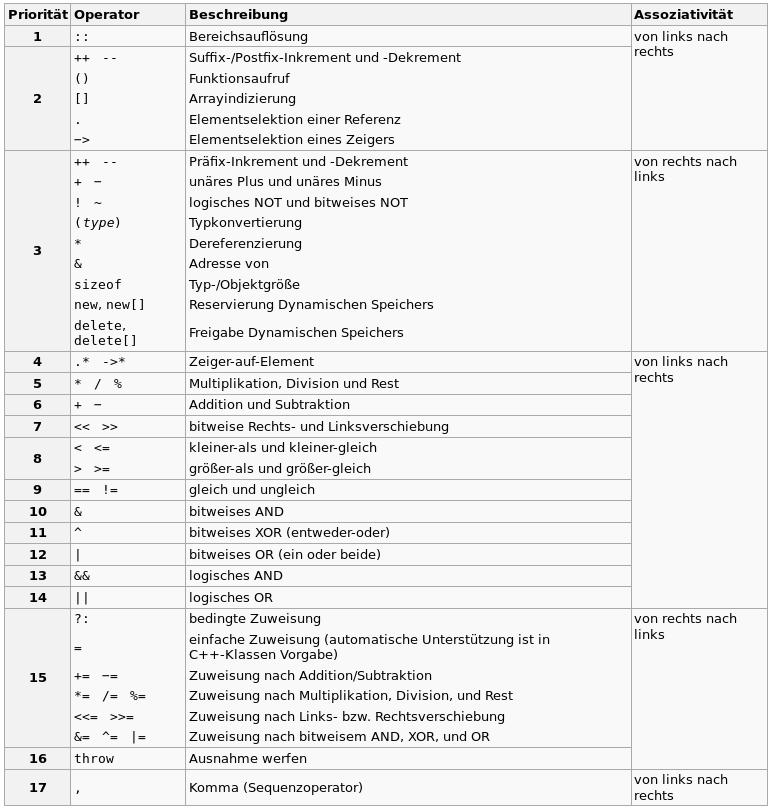
\includegraphics[width=0.9\linewidth]{images/operator}
\caption{Operatoren und deren Präzedenz}
\label{fig:operator}
\end{figure}

\subsubsection{Pre- und Postinkrement}
\begin{description}
	\item[Postinkrement, Postdekrement] \lstinline|x++, x--| = Lesen, dann ändern
	\item[Preinkrement, Predekrement] \lstinline|++x, --x| = Ändern, dann lesen
\end{description}

\subsection{Datentypen}
\begin{itemize}
	\item In C++ sind alles \textbf{Wertetypen}
	\item Im Gegensatz zu Java ist der Speicherverbrauch von Datentypen nicht fix, sondern Prozessorabhängig
	\item Short und Int sind minimal 16Bit gross, Long minimal 32 Bit und long long minimal 64 Bit.
	\item Es gibt keine unsigned Fliesskommatypen
	\item Es gilt 1 == sizeof(char) <= sizeof(short) <= sizeof(int) <= sizeof(long) <= sizeof(long long). 
	\item und float <= double <= long double
	\item Die konvertierung der Datentypen geschieht erst nach der Operation auf der rechten Seite der =.
\end{itemize}
\begin{table}[h]
	\centering
	\begin{tabu} to \linewidth {X l X}
		\toprule 
		Wertetype & Beispiele und Literale & Beschreibung \\
		\midrule
		void &  & der leere Typ \\
		bool & false = 0 und true= n $\neq$ 0  & Wird als Integer interpretiert (default = 1) \\
		char / unsigned char & \lstinline|'a', '\\n', '\\x0a'| & Wird als Integer interpretiert \\
		char array & \lstinline|\"ab\"| & \\
		short &  & \\
		int & \lstinline|1, 052(octal), 0x2A(hex)| &  \\
		long & \lstinline|42L| &  \\
		long long & \lstinline|5LL| &  \\
		unsigned short, \newline unsigned int, \newline unsigned long, \newline unsigned long long & \lstinline|1u, 42ul, 0xFULL| &  \\
		float & \lstinline|0.f|  &  \\
		double & \lstinline|.33| & default \\
		long double &  \lstinline|0.33L| &  \\
		\bottomrule 
	\end{tabu} 
	\caption{Wertetypen in C++}
\end{table}

\subsubsection{Signed und Unsigned}
Der Wertebereich von Ganzzahlen und Gleitkommazahlen ist implementationsabhängig und kann somit nicht fix angegeben werden. Bei den folgenden angaben ist $n$ = Anzahl Bits im Speicher
\begin{description}
	\item[signed (Standard)] \hfill \\
	Mit Vorzeichen: Wertebereicht $(-\frac{2^n}{2}) \text{ bis } (\frac{2^n}{2} - 1)$ (Wie in Java implizit signed)
	\item[unsigned] Ohne Vorzeichen: Wertebereich $0 \text{ bis } 2^n -1$
\end{description}

\subsubsection{Ganzzahlen}
\begin{itemize}
	\item C++ übernimmt eine automatische Typ Conversion.
	\item Bei Ganzzahldivisionen wird der Kommateil einfach abgeschnitten
	\item Lokale Integer Variablen werden standardmässig mit 0 initialisiert
	\item Teilen von Ganzzahlen durch 0, resultiert in \lstinline|undefined behavior| (Ausnahme Modulo)
\end{itemize}

\subsubsection{Gleitkommazahlen}
\begin{itemize}
	\item Es sollte immer Double verwendet werden
	\item NaN und (+/-)Inf sind gültige Werte für eine Gleitkommazahl
	\item Double Division durch 0 ergibt immer (+/-) \textbf{inf} 
	\item Double Variablen können nicht in Integer gespeichert werden, da sie mehr Speicher benötigen
	\item Lokale double Variablen werden standardmässig mit 0 initialisiert
	\item 0.0 / 0 = \textbf{NaN} 
\end{itemize}

\subsubsection{NaN} 
\begin{itemize}
	\item NaN Vergleiche geben immer false
	\item sqrt(-1) = NaN (Komplexes Resultat = NaN)
\end{itemize}

\subsection{Scopes}
\begin{enumerate}
	\item Global scope
	\item Named namespaces (können verschachtelt werden)
	\item Anonymous namespace (Vesteckt name vor dem Linker)
	\item Class scope (Members)
	\item Function scope (Parameter)
	\item Block scope (lokale Variablen)
	\item Temporaries (Resultate von Ausdrücken)
\end{enumerate}

\subsubsection{Shadowing}
Es ist möglich Parametervariablen zu überdecken. Dies sollte aber wenn möglich unterlassen werden, da es zu unübersichtlichem Programmcode führt.

\subsection{Namespaces}
\begin{itemize}
	\item Namespaces erstellen einen eigenen Scope mit welchem Nameskollision verhindert werden können. 
	\item Namespaces erlaubes es, den gleichne Namen in verschiedenen Namespaces zu verwenden.
	\item Der Namespace muss mit dem zweifachen Doppelpunkt Prefix verwendet werden
	\item Globaler namespace wird mit Doppelpunkten gekennzeichnet \lstinline|::separator, ::read()|
	\item \lstinline|using| Keyword niemals in Header File verwenden, sondern möchlichst lokal
	\item Mit \lstinline|using| können der Namespace weggelassen werden.
	\item Überladene Funktionen sollten immer im gleichen Namespace sein. Bekannte Funktionen wie z.B \lstinline|min()| sollten in ein eigenen Namespace gepackt werden, da sie ansonsten die \lstinline|min()| Funktion des Standard Namespace überladen.
	\item Funktionen werden immer im Namespace der Parameter gesucht. Möchte man das die eigenen Funktion aufrufen, muss der Namespace angegeben werden.
	\item \lstinline|using namespace| sollte nicht verwendet werden
\end{itemize}
\begin{lstlisting}[language=C++]
namespace demo {
	void foo(); //1
	namespace subdemo {
		void foo(); // 2
	} // subdemo
} // demo

namespace demo { // extends other namespace 'demo'
	void bar() {
		foo(); // 1
		subdemo::foo(); // 2
	}
}

void demo::foo() { // definition of 1
}

{
// anonymous namespace
// functions declared here, can not be called outside this file
// for helper functions, helper types, constants: used to hide members
}

using demo::subdemo::foo // single class or function
using namespace demo::subdemo // complete namespace

// example for using
using std::string;
string s{"no std::"};
\end{lstlisting}


\clearpage


\subsection{Unqualifizierte Namensauflösung / Argument Dependent Lookup}
Wenn der Typ des Funktionsargument im gleichen Namespace wie die Funktion ist, kann der Namespace weggelassen werden. Dies ist inbesondere bei den Operatoren wichtig. Das Lookup greift nur bei unqualifizierten Namen (ohne Angabe des Namspaces)
\begin{figure}[h]
\centering
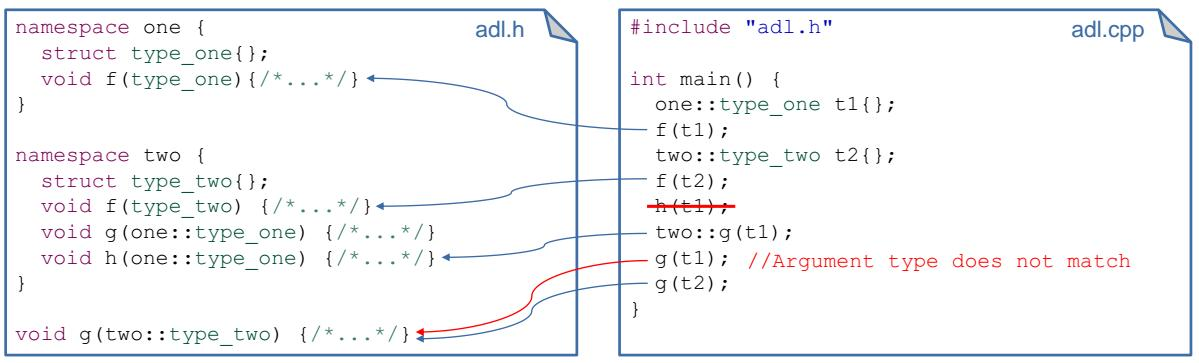
\includegraphics[width=0.9\linewidth]{images/adl_examples}
\caption{Argument Dependent Lookup}
\label{fig:adlexamples}
\end{figure}

\subsection{Alias / Using}
Mit dem Keyword \lstinline|using| kann ein Alias gesetzt werden. 
\begin{lstlisting}[language=C++]
using name=type;

// example
using input=std::istream_iterator<std::string>;
input eof{}
\end{lstlisting}

\subsection{Casting}
Casting sollte wenn möglich vermieden werden. In wenigen Fällen ist es aber unumgänglich und dann sollte man den \lstinline|static_cast| der C Variante mit den runden Klammern vorziehen.
\begin{lstlisting}
// bad
std::abs(index) > (int) this->size()) 

// good
std::abs(index) > static_cast<int>(this->size())
\end{lstlisting}

\clearpage

\newpage

\subsection{Kontrollstrukturen}
\subsubsection{Switch Case}
Switch Case funktioniert nur für Ganzzahlen
\begin{lstlisting}[language=C++]
void testSwitchCase(int weekDay) {
	switch (weekDay) {
		case 1:
		break;
		case 2:
		break;
		default:
		break;
	}
}
\end{lstlisting}

\subsubsection{For-Each}
\begin{lstlisting}[language=C++]
#include <string>
#include <vector>
#include <algorithm>

#include <iterator>
#include <iostream>

void testForEach(std::vector<std::string> const & items, std::ostream & out) {
	std::for_each(begin(items), end(items), [&out](auto s){
		out << s;
	});
}
int main() {
	std::vector<std::string> items{};
	items = {"abc","de","efg","hijk"};
	
	testForEach(items, std::cout);
	
	// implicit
	return 0;
}
\end{lstlisting}


\section{Variablen}
\begin{itemize}
	\item Variablen beginnen immer mit einem Kleinbuchstaben 
	\item Lokale Variablen müssen wie in Java immer mit einem Default Wert deklariert werden! (Geschweifte Klammern oder = bei \lstinline|auto| Variablen)
	\item Globale Variablen sollten nie verwendet werden.
	\item Es sollten keine veränderbaren globale Variablen deklariert werden
	\item Eine Variable sollte so nahe wie möglich bei dem Ort wo sie benötigt wird, deklariert werden.
	\item Variablen sind standardmässig Value Types und und werden somit bei der Definition auf dem Stack alloziert.
	\item Globale, veränderbare Variablen sollten vermieden werden, da sie schwer zu testen sind und beim Multithreading Probleme bereiten.
\end{itemize}
\begin{lstlisting}[language=C++]
<type> <name> { <default-value> }

int i{42}
int &ri{i} // must initialize ref
int const &cri{i}; // const alias
int const &cr{6*7} // extend lifetime of 6*7
ri = 43 // changes i, ri only an lias
// --cri; // does not work, because of const
int &&rv{3*14}; // extends lifetime of 3*14
// int &&rvri{i} impossible
int &&rvri{std::move(i)}; // steal i's content
\end{lstlisting}

\subsection{Reference / Value}
\subsubsection{By Value}
\begin{itemize}
	\item Bei Zuweisungen bei value von vererbten Werten gibt es ein Object Slicing (\lstinline|x=a|) (Siehe Vererbung)
\end{itemize}

\subsubsection{By Reference}
\begin{itemize}
	\item Variablenzuweisungen \lstinline|by reference| machen nur bedingt Sinn.
\end{itemize}

\clearpage

\subsection{Const}
\begin{itemize}
	\item Const sollte so oft wie möglich verwendet werden.
	\item Const ist ähnlich wie das \lstinline|final| in Java, jedoch mit höherer Garantie dass eine Variable oder Memberfunktion nicht verändert wird
	\item Konstanten müssen initialisiert werden
	\item Das Const bei Memberfunktionen bezieht sich auf das this Objekt. Const Funktionen dürfen Inhalt von dem \lstinline|this| Objekt nicht verändern.
	\item Um Konstanten zur Compilezeit zu setzten muss man das Keyword \lstinline|constexpr| verwendet werden.
\end{itemize}

\begin{remember}{Const}{}
	Alle Variablen die nicht verändert werden, müssen const sein!
\end{remember}

\subsection{Auto}
Das Auto Keyword versucht automatisch den Typ zu bestimmen und zwar gemäss der Zuweisung bei der Deklaration.
\begin{lstlisting}[language=C++]
auto const m=4; //int
auto const s="Hello"s; // std:string
\end{lstlisting}

\subsection{Inline}
Wenn ein Member in Header definiert wird, muss die Definition inline sein. Dies sollte nur gemacht werden, wenn der Funktionsbody sehr kurz ist. Eine Inline Function erlaubt dem Compiler den Function Call Overhead weg zu optimieren.
\begin{lstlisting}[language=C++]
inline double square(double val) {
	return val * val;
}
\end{lstlisting}


\section{Funktionen}
\begin{itemize}
	\item Funktionen werden im lower Camel Case geschrieben
	\item Eine Funktion muss immer zuerst im Header File deklariert werden, bevor man sie verwenden kann
	\item Eine Funktion hat einen guten Namen, maximal 5 Parameter (besser 3) und erledigt genau eine Sache.
	\item Bei den Funktionsparameter ist die Aufrufreihenfolge nicht definiert (z.B Wenn der Funktionsparameter der Rückgabewert einer Funktion ist)
	\item Die Main Funktion gibt implizit 0 zurück
	\item Auto sollte nicht als Return Typ angegeben werden. Ausnahme sind Inline, Template oder Constexpr Funktionen in Header Files.
	\item Void sollte nicht als Funktionsparameter verwendet werden.
\end{itemize}
\begin{lstlisting}[language=C++]
// result type can be auto, but should not
result_type function_name(parameter_type parameter) {
	return return_variable;
}
\end{lstlisting}

\subsection{Default Arguments}
Default werde sollte erst bei der Deklaration gesetzt werden. Die Parameter mit einem Default werde, müssen nicht übergeben werden.
\begin{lstlisting}[language=C++]
void incr(int &var, unsigned delta=1) {}
\end{lstlisting}

\subsection{Reference / Value}
\subsubsection{Call by Value}
\begin{itemize}
	\item Parameter werden standardmässig als Wert (value) übergeben
	\item Es wird dabei eine Kopie des Parameters erstellt (Achtung: Grosse Objekte) $\rightarrow$ besser Refenz verwenden.
	\item \lstinline|ret_type f(type param){ .. }|
\end{itemize}

\subsubsection{Call by Reference}
\begin{itemize}
	\item Referenzen machen nur als Parameterübergabe Sinn, nicht aber bei Zuweisungen von lokalen Variablen.
	\item Referenz Parameter werden mit dem \& Prefix markiert (lvalue)
	\item RValue Referenzen werden mit dem \&\& Prefix markiert. RValue Referenzen verschieben den Inhalt
	\item Referenzen können \lstinline|const| sein. Speziell für grosse Objekte die nicht verändert werden.
	\item Niemals eine Referenz auf eine lokale Variable zurückgeben, da das Stackframe nach dem Methodenaufruf abgebaut wird! (Dangling Reference). \lstinline|int & my_func() { int n{42} return n;}|
	\item Das Orginal muss mindestens so lange leben wie die Referenz darauf.
	\item Referenzen könnnen zurückgegeben werden. \lstinline|int my_func(int &n) { return n; }|
\end{itemize}
\begin{lstlisting}[language=C++]
void askForName(std::ostream &out)
\end{lstlisting}

\begin{figure}[h]
\centering
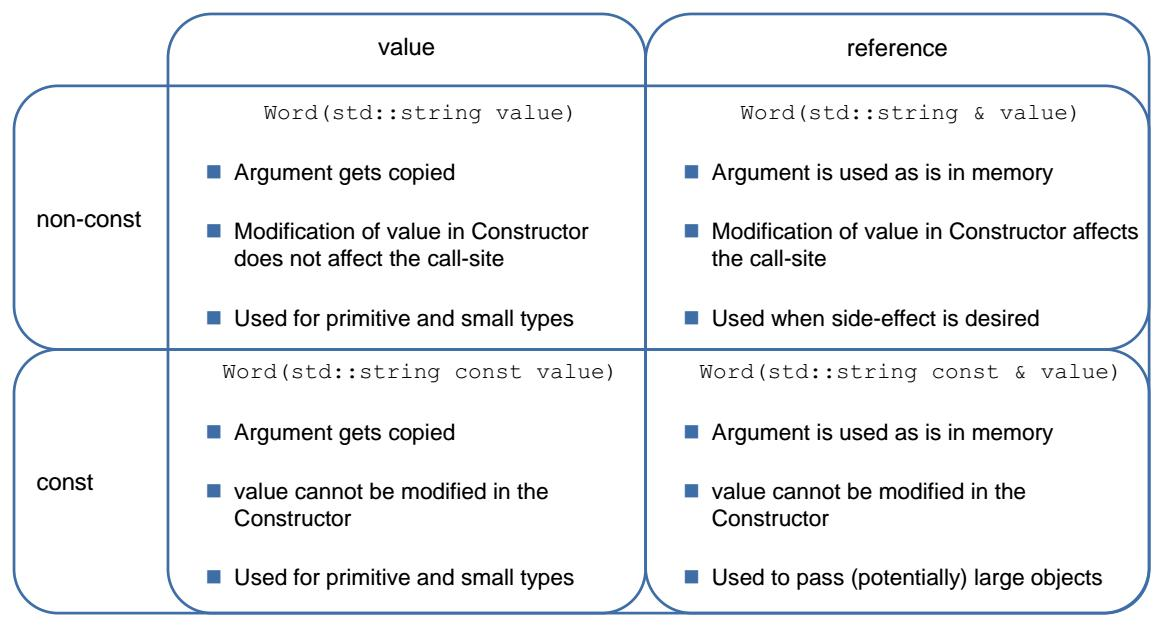
\includegraphics[width=0.7\linewidth]{images/val_ref_params}
\caption{Constructor und Function Parameter}
\label{fig:valrefparams}
\end{figure}



\subsection{Function Overloading}
Unter Function Overloading versteht man, dass mehrere Funktionen den selben Namen aber unterschiedliche Parameter haben. (Unterschiedliche Signatur)
\begin{lstlisting}[language=C++]
void incr(int& var);
int incr(int& var); // does not compile
void incr(int& var, unsigned delta);
\end{lstlisting}

\subsection{Template Function}
\begin{itemize}
	\item Funktions Templates werden normalerweise direkt im Header deklariert und implementiert
	\item Template Funktionen sind implizit inline
	\item Mit Templates können generische Funktionen geschrieben werden, damit es keine Probleme mit überladenen Funktionen gibt (mehrdeutigkeiten)
	\item Bei Mehrdeutigkeiten muss der Typ in den Spitzen-Klammern übergeben werden.
	\item Das \lstinline|typename| Keyword kann mit durch das Keyword \lstinline|class| ersetzt werden. (deprecated)
\end{itemize}
\begin{lstlisting}[language=C++]
template <typename T, typenmae U, etc.>

namespace CustomMin {
	// could be ambiguous
	inline int min(int a, int b){
		return (a < b)? a : b ;
	}
	inline double min(double a, double b){
		return (a < b)? a : b ;
	}
	
	// solution
	template<typename T> 
	T const& min(T const& a, T const& b){
		return (a < b)? a : b ;
	}
}

// call
min(1, 1);
min(2, 2)
min<doubl>(1, 2.0); // ambiguos without template

// char array mit unterschiedlichen laengen muessen explizit als string verglichen werden
MyMin::min<std::string>("Test", "Test2"); // std namespace already has a min function
MyMin::min("Test"s, Test2"s); // alternative variante
\end{lstlisting}


\subsubsection{Variable Parameter}
Wie in Java werden die drei Punkte für beliebig viele Parameter benutzt.
\begin{lstlisting}[language=C++]
template <typename...ARGS>
void variadic(ARGS...args){
	println(std::cout,args...);
}

// example
template<typename Head, typename... Tail>
	void println(std::ostream &out, Head const& head, Tail const& ...tail) {
	out << head;
	if (sizeof...(tail)) {
		out << ", ";
	}
	println(out,tail...); //recurse on tail
}
// base case
void println(std::ostream &out) {
	out << "\n";
}
\end{lstlisting}

\clearpage

\subsection{Funktionsparameter}
Alle Funktionen und Lamdas können als Parameter eine weiteren Funktion übergeben werden. Funktionen, Funktoren und Lamdas können in einem \lstinline|std::function<x(y)>| Objekt gespeichert werden.
\newpage

\begin{lstlisting}[language=C++]

// std::function definiert den Rueckgabe und Parameter Typ
std::function<bool(int)> apredicate{};

// member function pointer, wobei calc eine Methode einer Klasse ist
std::function<int (X const &,int)> const f{&X::calc};


void printfunc(double x, double f(double)){
	std::cout<< f(x);
}

double square(double d) {
	return d*d;
}

printfunct(1.0, std::atan);
printfunct(1.0, square);
printfunct(2.0, [](double x){return x*x;});
\end{lstlisting}

\subsection{Lamdas}
\begin{itemize}
	\item Lamdas können auch in Variablen geschrieben werden \lstinline|auto l = []{}; l();|
	\item Das kleinste Lamda wäre \lstinline|[]{}()|, wobei die ersten beiden Klammern das Funktionsobjekt sind und die runde Klammer der Aufruf.
	\item Der \lstinline|return_type| kann auch weggelassen wenn dieser \lstinline|void| oder konsistent ist.
	\item Das Lamda Capture kann verwendet werden, wenn das Lamda als Funktionsparameter übergeben wird und man trotzdem noch Variablen aus dem lokalen Context verwendetn möchte.
	\item Ein Predicate nimmt ein oder mehrere Parameter entgegen und gibt \lstinline|true| oder \lstinline|false| zurück.
\end{itemize}
\begin{lstlisting}[language=C++]
// return_type is optional
auto const l = [lamda_capture](parameters) -> return_type {
	statements;
};
// call
l(param);

// lamda campture
#include <functional>
void f(std::function<char(char)> function) {
	std::cout << function('a');
}
void main() {
	unsigned i{1};
	auto const g = [i](char c) -> {
		return std::toupper(c) + i;
	}
}
\end{lstlisting}

\subsubsection{Captures}
Es ist guter Stil explizit zu capturen. Es sind auch Kombination von Caputures möglich
\begin{itemize}
	\item $[=]$ - default implicit capture variables used in body by value  
	\item $[\&]$ - default capture variable used in body by reference 
	\item $[var=value]$ - introduce new capture variable with value 
	\item $[=,\&out]$ - capture all by copy, but out by reference 
	\item $[\&,=x]$ - capture all by reference, but x by copy/value 
\end{itemize}
Gecapturete Variablen sind standardmässig nicht veränderbar. Man muss sie also entweder \lstinline|mutable| definieren und per Referenz übergeben:
\begin{lstlisting}[language=C++]

std::vector<int> v;
int x{}; // memory for lambda below

// mutable
generate_n(std::back_inserter(v),10,[x=0]() mutable { 

// reference
generate_n(std::back_inserter(v),10,[&x]{
++x; return x*x;
});

class  make_squares{
int x{};
public:
int operator()() { ++x; return x*x; }
};

//...
generate(v.begin(),v.end(),make_squares{});
\end{lstlisting}


\subsubsection{Parameter}
\begin{itemize}
	\item Die Parameter können auch als \lstinline|auto| deklariert, wenn klar ist, welcher Typ übergeben wird.
\end{itemize}

\clearpage

\subsection{Functor}
Functoren sind Typen die eine bestimmte Operation zur Verfügung stellen. Funktoren haben den call Operator überladen haben. Lamdas arbeiten intern mit Functoren. Die \lstinline|operator()| Funktion kann theoretisch beliebig oft überladen werden.
\begin{lstlisting}[language=C++]
struct Accumulator {
	int count{0};
	int accumulated_value{0};
	
	// two parentheses required
	// Wenn die Funktion keine Memeber veraendert, sollte sie const sein!
	void operator()(int value) {
		count++;
		accumulated_value += value;
	}
	int average() const;
	int sum() const;
};

// Use of Accumulator. Return Average of accumalted Sum
int average(std::vector<int> values) {
	Accumulator acc{};
	for(auto v : values) { acc(v); }
	return acc.average(); 
	
	// rsp. mit einem Algorithmus
	return std::for_each(begin(values), end(values), acc).average();
}
\end{lstlisting}


\subsection{Standard Funktoren}
Häufig gebrauchte Funktoren werden von der Functional Libary zur Verfügung gestellt. Associative Container Typen können die Standardfunktion zur Initialisierung übergeben werden.
\begin{lstlisting}[language=C++]
#include <functional>
// arithmetic
plus<>{}
minus<>{}
divides<>{}
multiplies<>{}
modules<>{}
logical_and<>{}
logical_or<>{}
// unary
negate<>{}
logical_not<>{}
// binary
less<>{}
less_equal<>{}
equal_to<>{}
greater_equal<>{}
not_equal_to<>{}

// example
transform(v.begin(), v.end(), v.begin(), v.begin(), std::multiplies<>{})

// sort set in reverse order
std::set<int, std::greater<>> reverse_int_set{};
\end{lstlisting}



\section{Klassen}
Klassen und Structs werden immer in Header Files definiert. Die Implementierung kann dann in einem beliebigen File stattfinden.
\begin{itemize}
	\item Bei einer class sind alle Member implizit private
	\item Klassenmember sind implizit \lstinline|inline|!
	\item Nach der Klassen Definition muss ein Semikolon stehen!
	\item Membervariablen sollten nie für die Kommunikation zwischen Memberfunktionen missbraucht werden.
	\item Zugriff auf die aktuelle Instanz ist via \lstinline|this->member| rsp. \lstinline|this->memberfunction()|
	\item Das \lstinline|this| Objekt ist ein Pointer und muss nur verwendet werden, wenn der Name des Membervariable gleich einer lokalen Variable ist.
	\item Wenn man das wirkliche \lstinline|this| Objekt übergeben will, muss der Pointer mittels \lstinline|*this| dereferenziert werden.
	\item Memberfuntionen sollten wenn möglich \lstinline|const| sein, solange sie das \lstinline|this| Objekt nicht verändern.
\end{itemize}

\begin{lstlisting}[language=C++, caption=A good Class]
class <GoodClassName> {
	<member variables>
	<constructors>
	<member function>	 							
};	
\end{lstlisting}


\begin{lstlisting}[language=C++, caption=Klassentyp im Header File]
#ifndef DATE_H_
#define DATE_H_
class Date {

	int year, month, day;
	bool isValid();
	
public:
	Date() = default;
	explicit Date(int year, int month, int day)
		: year{year}, month{month}, day{day} {/*...*/}
	
	static bool isLeapYear(int year) {/*...*/}

private:
	bool isValidDate() const {/*...*/}
};

#endif /* DATE_H_ */
\end{lstlisting}

\begin{lstlisting}[language=C++, caption=Implementierung des Klasse ]
#include "Date.h"
Date::Date(int year, int month, int day)
	: year{year}, month{month}, day{day} { 
	
		if (!isValidDate()) {
			throw std::out-of_range{"invalid date"};
		}
	}

Date::Date() : Date{1,1,1980} {} // default constructor

Date(Date const & other) : Date{other.day, other.month, other.year} {} // copy constructor

bool Date::isLeapYear(int year){
	/*...*/
}

bool Date::isValidDate() const
{
	// acess member
	()*this).member
	this -> member
}
\end{lstlisting}

\begin{lstlisting}[language=C++, caption=Verwendung des Klasse ]
#include "Date.h"

void foo() {
	Date today{19.10.2016};
	
	auto thursday{today.tomorrow()};
	
	Date::isLeapYear(2016);
}
\end{lstlisting}

\subsection{Struct}
\begin{itemize}
	\item Bei einer Struct sind alle Member implizit public
	\item Nach dem Kompilieren ist die Struct aber genau gleich wie die Klasse
\end{itemize}


\subsection{Sichtbarkeiten}
Die Visibility gilt für einen bestimmten Bereich
\begin{description}
	\item[private] Nur innerhalb der Klasse gültig (and friends)
	\item[protected] Auch sichtbar in Subklassen
	\item[public] Sichtbar für alle
\end{description}

\clearpage

\subsection{Konstruktoren}
\begin{itemize}
	\item Anstatt der Default Initialisierung können die Member Variablen auch schon im Header File initialisiert werden (NSDMI: Non Static Data Member Initializers)
\end{itemize}
\begin{lstlisting}[language=C++, caption=Konstruktoren]
<class name> ( <parameters> ) : <initializer-list> {}

// default constructor
<class name> ()
Date::Date() : year{2016}, month{10}, day{26} {}
Date d{}; // call

// copy constructor
<class name> ( <class name> const & ) 
Date(Date const &)
Date d2{d}; // call

// move constructor (C++ Advanced)
<class name> ( <class name> &&) 
Date(Date &&)
Date d2{std::move(d)};

// typeconversion constructor 
// explicit avoids implicit conversion!
// const & avoids unnecessary copy
explicit <class name> ( <other type> const & )
explicit Date(std::string const &);
Date d{"19/10/2016"s};

// Examples
Date{16,10,2016};
Date(int day, int month, int day) :
localDay{day}, localMonth{day}, localYear{Year} { /* .. */}

// inherit constructor from base class
using std::set<T, COMPARE>::set;
\end{lstlisting}

\subsection{Defaulted Constructors}
Damit der Default Konstruktor im *.cpp File nicht mehr angegeben werden muss, kann er direkt im Header File als Default deklariert werden. Dies ist auch für den Copy und Move Konstruktor möglich. Mit dem \lstinline|default| Keyword wird ebenfalls der Default Konstrutor redefiniert, wenn nur ein Konstruktor mit Parameter angegeben ist.
\begin{lstlisting}[language=C++, caption=Defaulted Constructors]
#ifndef DATE_H_
#define DATE_H_
class Date {
	int year{9999}, month{12}, day{31};
	//...
	Date() = default;
	Date(int year, int month, int day);
};
#endif /* DATE_H_ */
\end{lstlisting}

\subsection{Factory Functions}
Eine Factory Methode beginnt meist mit \lstinline|make| oder \lstinline|create|
\begin{lstlisting}[language=C++, caption=Factory Functions]
Date make_date(std::istream & in) {
	try {
		return Date{in};
	} catch (std::out_of_range const &) {
		return Date{9999, 12, 31}; // default date
	}
}
\end{lstlisting}


\subsection{Destruktor}
Im Destruktor darf nie eine Exception geworfen werden. 
\begin{lstlisting}[language=C++, caption=Destruktor]
	~Date(); // implizit
\end{lstlisting}

\subsection{Vererbung}
Die Art der vererbung kann wieder mit den Sichtbarkeits Modifier gesteuert werden. (private, protected, public)
\begin{lstlisting}[language=C++, caption=Konstruktoren]
class Base { 
	private:
		int onlyInBase;
	protected:
		int baseAndInSubclasses;
	public: 
		int everyone;
};

class Sub : public Base {
	
};
\end{lstlisting}

\subsection{Statische Member}
\begin{itemize}
	\item Die \lstinline|static| Definition ist nur im Header File
	\item Statische Member verfügen über kein \lstinline|this| Objekt. D.h sie gehören zu der Klasse und nicht zu deren Instanzen.
	\item Statische Member (in der Implementierung) können nicht \lstinline|const| sein. Im Headerfile jedoch schon: \lstinline|static const int zero{0};|
	\item Können direkt via \lstinline|<classname>::<member>();| aufgerufen werden
\end{itemize}

\clearpage


\subsection{Klassen Templates}
\begin{hint}{Prüfung}{}
	Klassen Template kommen bestimmt an der Prüfung und geben viel Punkte.
\end{hint}
\begin{itemize}
	\item Template Klassen werden komplett im Header File definiert
	\item Klassentemplates liefern Typen mit \textbf{Compile-time} Parameter
	\item Man muss \lstinline|typename| verwenden, wenn das Element direkt oder indirekt vom Template Parameter abhängt.
	\item Als Template Parameter können Typen (typename), Kostanten oder weitere Templates (template) übergeben werden.
	\item T als Übergabeparameter darf nicht void sein
	\item T als Rückgabewert muss kopierbar (oder movebar) sein	(da der Vector Wertetypen enthält, keine Referenzen)
	\item Memberfunktionen die nie benutzt werden, werden bei Template Klasse nie kompiliert.
	\item Auf vererbten Member sollte immer mit \lstinline|this->member| oder \lstinline|[class-name]::member| zugegriffen werden.
\end{itemize}

\subsection{Terminologie}
\begin{figure}[h]
	\centering
	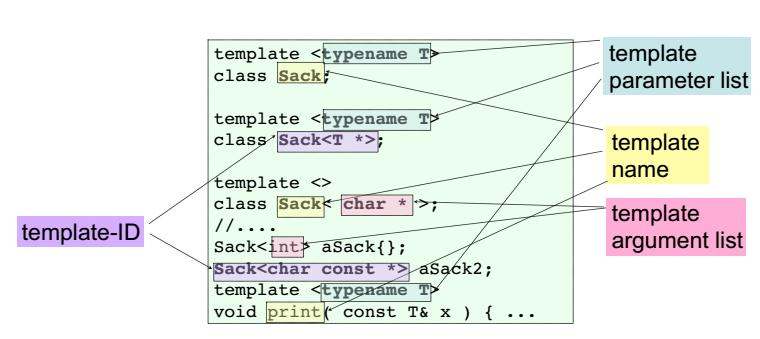
\includegraphics[width=0.7\linewidth]{images/class_template_terminologie}
	\caption{Klassen Template Initialisierung}
	\label{fig:classtemplateterminologie}
\end{figure}

\clearpage

\begin{lstlisting}[language=C++, caption=Klassen Templates]
template <typename T> class [classname];
template <typename T> class [classname]<T *>;
template <> class [classname]<char *>;


template <typename T> class Sack {
	using SackType = std::vector<T>;
	// inherit constructor from base class
	using std::set<T, COMPARE>::set;
	using size_type = typename SackType::size_type;
	
	SackType theSack{};

public:
	bool emtpy() const {return theSack.empty(); }
	size_type size() const { return theSack.size(); }
	void putInto(T const & item) { theSack.push_back(item); }
	
	// forward declaration	
	T getOut();
}

template <typename T> inline T Sack<T>::getOut() {
	if (! size() ) {
		throw std::logic_error{"empty sack"};
	}
	auto index = static_cast<size_type>(rand()%size());
	T retval{theSack.at(index)};
	theSack.erase(theSack.begin()+index);
	return retval;
}


// specialization
template <typename T> class Sack;

template <> class Sack<char const *> {
	typedef std::vector<std::string> SackType;
	typedef SackType::size_type size_type;
	SackType theSack;
public:
	// no explicit ctor/dtor required
	bool empty() { return theSack.empty() ; }
	size_type size() { return theSack.size();}
	void putInto(char const *item) { theSack.push_back(item);}
	std::string getOut() {
		if (! size()) {
			throw std::logic_error{"empty Sack"};
		}
		std::string result=theSack.back();
		theSack.pop_back();
		return result;
	}
};
\end{lstlisting}

\clearpage

\subsubsection{Pointer} 
Pointer sollten nicht verwendet werden.
\begin{lstlisting}[language=C++, caption=Klassen Templates Pointer]
// may the only exception
Sack<char const *> shouldkeepStrings;

// Prohibit pointers
template <typename T> struct Sack<T*> {
	~Sack()=delete;
}
\end{lstlisting}

\subsubsection{Konstruktor}
\begin{lstlisting}[language=C++, caption=Klassen Templates Pointer]
template <typename T> class Sack {
	using SackType=std::vector<T>;
	using size_type=typename SackType::size_type;
	SackType theSack{};
	
public:
	Sack()=default;

	template <typename ITER> 
		Sack(ITER b, ITER e):theSack(b,e){}
}
\end{lstlisting}

\begin{lstlisting}[language=C++]
struct B1 {
	B1(int);
};
struct D1 : B1 {
	using B1::B1;
	// The set of candidate inherited constructors is 
	// 1. B1(const B1&)
	// 2. B1(B1&&)
	// 3. B1(int)
	
	// D1 has the following constructors:
	// 1. D1()
	// 2. D1(const D1&) 
	// 3. D1(D1&&)
	// 4. D1(int) <- inherited
};

struct B2 {
	B2(int = 13, int = 42);
};
struct D2 : B2 {
	using B2::B2;
	// The set of candidate inherited constructors is
	// 1. B2(const B2&)
	// 2. B2(B2&&)
	// 3. B2(int = 13, int = 42)
	// 4. B2(int = 13)
	// 5. B2()
	
	// D2 has the following constructors:
	// 1. D2()
	// 2. D2(const D2&)
	// 3. D2(D2&&)
	// 4. D2(int, int) <- inherited
	// 5. D2(int) <- inherited
};

\subsection{Template Template Parameter}
\begin{lstlisting}[language=C++, caption=Klassen Templates Pointer]
template <typename T, template<typename...> class container=std::vector> class Sack {
	
}

Sack<int,std::list> listsack{1,2,3,4,5};
\end{lstlisting}



\section{Enums}
\begin{itemize}
	\item Enumerationen werden verwendet für Typen die nur wenige Werte halten.
	\item Jedes Enum Feld kann leicht in einen int konvertiert werden, beginnend bei 0. Die int Werte können auch manuell mit = beliebig zugewiesen werden.
	\item Mit dem \lstinline|class| Keyword (Scoped Enum) ist der Enum Typ nicht ausserhalb des Namespaces sichtbar. Beim normalen unscoped Enum jedoch schon
	\item Die Namen des Enums können standardmässig nicht ausgegeben werden. Dazu muss man eine Lookuptable mit einem String Array anlegen.
\end{itemize}

\begin{lstlisting}[language=C++, caption=Enum]
enum [class] <name> { 
	<enumerators>
};

enum class day_of_week {
   //0     1      2      3      4      5      6
	Mon, Tue, Wed, Thu, Fri, Sat, Sun
	
	//operator overload
	day_of_week operator++(day_of_week & aDay) {
		int day = (aDay + 1) % (Sun + 1); // convert to int
		aDay = static_cast<day_of_week>(day);
		return aDay;
	}
};

// ex2: specify type with inheritance
enum class launch_policy : unsigned char {
	sync=1, async=2, gpu=4, process=8, none=0
};

// v3
enum Color { red, green, blue };
Color r = red;
switch(r) {
	case red  : std::cout << "red\n";   break;
	case green: std::cout << "green\n"; break;
	case blue : std::cout << "blue\n";  break;
}
\end{lstlisting}

\section{Operator Overloading}
\begin{itemize}
	\item Operatoren können für Klassen, Structs und Enums überladen werden
\end{itemize}
\begin{lstlisting}[language=C++, caption=Mögliche Operatoren zum Überladen]
<returntype> operator<op>(<parameters>);

// overloadable operators
+ - * / % ^
& | ~ ! , =
< > <= >= ++ --
<< >> == != && ||
+= -= /= %= ^= &=
|= *= <<= >>= [] ()
-> ->* new new [] delete delete []

// non overloadable operators
:: .* . ?
\end{lstlisting}

%TODO: Braucht es hier die erste Date-Definition (siehe auch nächste Sektionen)
\begin{lstlisting}[language=C++, caption=Operator Overloading]
class Date {
	int year, month, day; //private 
	bool operator<(Date const & rhs) const {
		return year < rhs.year ||
		(year == rhs.year &&
		(month < rhs.month || (month == rhs.month && 
		day == rhs.day)));
	}
}

#include <iostream>
class Date {
	int year, month, day; // private
	public:
		// Memberfunktionen
		std::ostream & print(std::ostream & os) const {
			os << year << "/" << month << "/" << day;
			
			// return stream obj, to allow output to chain values
			return os;
		}
		
		std::istream & read(std::istream & is) {
			int year{-1}, month{-1}, day{-1};
			char sep1, sep2;
			//read values
			is >> year >> sep1 >> month >> sep2 >> day;
			try {
				Date input{year, month, day};
				//overwrite content of this object (copy-ctor)
				(*this) = input;
				//clear stream if read was ok
				is.clear();
			} catch (std::out_of_range & e) {
				//set failbit
				is.setstate(std::ios::failbit | is.rdstate()); 
			}
			return is;
		}
};
	
// Inline Funktionen die die Member aufrufen
inline std::ostream & operator<<(std::ostream & os, Date const & date){
	return date.print(os);
}

inline std::istream & operator>>(std::istream & is, Date & date) {
	return date.read(is);
}

// simplyfied solution with tuples
#include "Date.h"
#include <tuple>
bool Date::operator<(Date const & rhs) const {
	return std::tie(year, month, day) < std::tie(rhs.year, rhs.month, rhs.day);
}
\end{lstlisting}

\subsection{Pre- Postfix Incrementation Overload}
\begin{lstlisting}[language=C++]
enum dayOfWeek {
	Mon, Tue, Wed, Thu, Fri, Sat, Sun
};

// Prefix
dayOfWeek operator++(dayOfWeek & aday) {
	int day = (aday + 1) % (Sun + 1);
	aday = static_cast<dayOfWeek>(day);
	return aday;
}

// Postfix (Int is obsolete, just for signature diversity)
dayOfWeek operator++(dayOfWeek & aday, int) {
	dayOfWeek ret{aday};
	if (aday == Sun) { 
		aday = Mon;
	} else {
		aday = static_cast<dayOfWeek>(aday + 1);
		return ret;
	}
}
\end{lstlisting}

\clearpage

\subsubsection{Grösser / Kleiner als / gleich Overload}
\paragraph{Wörter vergleichen} \hfill \\
\begin{lstlisting}[language=C++]
// word.h
class Word {
private:
	std::string word;

public:
	Word() = default;
	Word(std::string word);

	std::ostream & print(std::ostream & os) const;
	std::istream & read(std::istream & is);

	bool operator<(Word const & rhs) const;
};

inline std::ostream & operator<<(std::ostream & os, Word const & word) {
	return word.print(os);
}

inline std::istream & operator>>(std::istream & is, Word & word) {
	return word.read(is);
}

inline bool operator>(Word const & lhs, Word const & rhs) {
	return rhs < lhs;
}

inline bool operator>=(Word const & lhs, Word const & rhs) {
	return !(lhs < rhs);
}

inline bool operator<=(Word const & lhs, Word const & rhs) {
	return !(rhs < lhs);
}

inline bool operator==(Word const & lhs, Word const & rhs) {
	return !(lhs < rhs) && !(rhs < lhs);
}

inline bool operator!=(Word const & lhs, Word const & rhs) {
	return !(lhs == rhs);
}

// word.cpp
bool Word::operator<(Word const & rhs) const {
	return std::lexicographical_compare(word.begin(), word.end(), rhs.word.begin() ,rhs.word.end(), [](char lhs, char rhs) {
		return std::tolower(lhs)<std::tolower(rhs);
	});
}
\end{lstlisting}

\section{Fehlerbehandlung}
Es gibt fünf Möglichkeiten der Fehlerbehandlung
\begin{enumerate}
	\item Fehler ignorieren wobei undefined behaviour möglich ist (z.B vector[0])
	\item Default Wert retournieren (z.B Beim Einlesen des Hostnamen ''localhost'')
	\item Fehlercode oder Fehlerwert zurückgeben (\lstinline|bool| oder -1 (falls Wert nur positiv))
	\item Statusbit setzen (Streams good(), fail(), bad())
	\item Exception werfen	
\end{enumerate}

\subsection{Exceptions}
\begin{itemize}
	\item \lstinline|std::exception| ist die Basisklasse aller Exceptions
	\item In der Memberfunktion \lstinline|what()| steht die Fehlerbeschreibung
	\item Throw by value, catch by const reference!
	\item Es könnten beliebige Werte Typen (\textbf{value} types) geworfen werden
	\item Das Keyword \lstinline|noexcept| garantiert, dass eine Memberfunktion nie eine Exception wirft. Tut sie dies doch, terminiert das Programm.
	\item Schreibt man eigene Exceptions, kann der Ausdruck ''Exception'' im Namen der Exception weggelassen werden
\end{itemize}
\begin{lstlisting}[language=C++]
#include <stdexcept> // contains some subclass of std::exception (std::logic_error or std::invalid_argument)

throw std::logic_error("message");

try {
.. 
} catch ( std::logic_error const & e) { 
e.what();
throw; // re-throw
} catch ( ... ) {
// catchs all exceptions, because there is no specific super type
}

int minimum (int a, int b) noexcept {
	return a<b?a:b;
}
\end{lstlisting}


\section{Streams IO}
\begin{itemize}
	\item In den Header Files sollte die Vorwärtsdeklaration \lstinline|#include <iosfwd>| verwendet werden. In den Source Files für \lstinline|std::cin| und \lstinline|std::cout| \lstinline|#include <iostream>| und falls nur einer der beiden Stream Objekte benötigt wird, \lstinline|#include <istream>| rsp. \lstinline|#include <ostream>|. Die letzten beiden Includes beinhalten kein \lstinline|std::cin| und \lstinline|std::cout|.
	\item Innerhalb von Main verwendet man std::cin und std::cout und die jeweiligen Shift Operatoren $>>$ und $<<$
	\item std::istream Objekte geben false zurück, falls sie sich in einem invaliden Status befinden.
	\item std::endl flushed gepufferten Out Stream. Man sollten deshalb besser das einfach \lstinline|'\n'| verwenden.
\end{itemize}

\subsection{Bits}
Auf der linken Seite der Tabelle sind alle möglichen Bit zustände aufgelistet. Auf der rechten Seite stehen die Rückgabewerte der einzelnen Abfragefunktionen.
\begin{figure}[h]
\centering
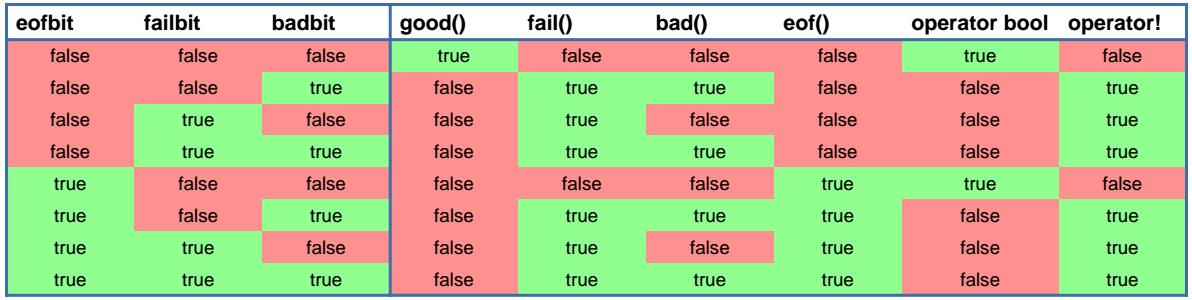
\includegraphics[width=\linewidth]{images/stream_bits}
\caption{Stream Bits}
\label{fig:streambits}
\end{figure}
\begin{figure}[h]
	\centering
	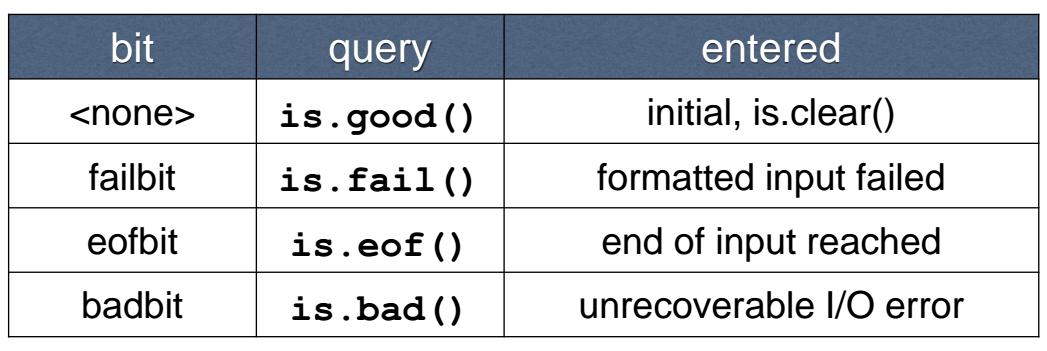
\includegraphics[width=0.7\linewidth]{images/stream_state_bits}
	\caption{Input Stream State Bits}
	\label{fig:streamstatebits}
\end{figure}


\clearpage

\subsection{Input}
\begin{lstlisting}[language=C++, caption=Simple Input Stream]
#include <istream>

int readInteger(std::istream& in) {
	while(in) {
		int mynumber{-1};
		if (in >> mynumber) {
			return mynumber;
		}
		in.clear(); // renive fail flag
		in.ignore(); // ignore one char
	}
	return -1;
}

int readString(std::istream & in) {
	while(in) {
		std::string line{};
		std::getline(in, line);
		std::istringstream is{line};
	}
	
	while (is.peek() != EOF) {
		if (std::isalpha(is.peek())) {
			word.push_back(is.get());
		} else {
			break;
		}
	}
}
\end{lstlisting}



\subsection{Output}
\begin{lstlisting}[language=C++, caption=Formatting Output]
#include <iostream>
#include <iomanip>

std::cout << std::[oct|hex|dec] << 24 << '\t'
std::cout << std::setw(10) << 24 // set width of next output line

double const pi{std::acos(0.5)*3}
std::cout << std::setprecision(4) << pi
std::cout << std::scientific << pi
std::cout << std::fixed << pi * 1e6
\end{lstlisting}


\clearpage

\subsection{Manipulatoren}
Für die Formatierung der Ausgabe kann man einer breiten Auswahl an Manipulatoren gebrauch machen.
\begin{table}[h]
	\centering
	\begin{tabu} to \linewidth {l l X}
		\toprule 
		Manipulator & Input / Output & Beschreibung \\
		\midrule
		\lstinline|std::dec| & beides & sets integer format to decimal \\
		\lstinline|std::oct| & beides & sets integer format to octal \\
		\lstinline|std::hex| & beides & sets integer format to hexadecimal \\
		\lstinline|std::showpos| & beides & show plus sign for positive numbers \\
		\lstinline|std::noshowpos| & beides & do not show plus sign \\
		\lstinline|std::showbase| & beides & sets integer format to show base \\
		\lstinline|std::noshowbase| & beides & sets integer format to not show base \\
		\lstinline|std::uppercase| & beides & use upper case for hex digits, exponent etc \\
		\lstinline|std::nouppercase| & beides & use lower case for hex digits, exponent etc \\
		\lstinline|std::boolalpha| & beides & use  ''true''  and  ''false''  for  bool \\
		\lstinline|std::noboolalpha| & beides & use 1 and 0 for bool i/o \\
		\midrule
		\lstinline|std::setw(n)| & beides & sets  next  field  width  to  n,  non sticky \\
		\lstinline|std::setfill(c)| & output & sets output field fill character \\
		\lstinline|std::left| & output & output   towards   the   left   in a wider field, fill character on the right \\
		\lstinline|std::right| & output & output  towards  the  right  in  a wider field, fill character on the left \\
		\lstinline|std::internal| & output & fill character between sign/base and number \\
		\midrule
		\lstinline|std::scientific| & beides & sets  floating  point  format  with exponent \\
		\lstinline|std::fixed| & beides & sets  fixed  floating  point  format without exponent \\
		\lstinline|std::defaultfloat| & beides & sets default floating point format \\
		\lstinline|std::setprecision(n)| & beides & sets significant or  fractional number of digits \\
		\lstinline|std::showpoint| & output & include floating point always \\
		\lstinline|std::noshowpoint| & output & omit floating point if possible \\
		\midrule
		\lstinline|std::flush| & output & flush buffered output \\
		\lstinline|std::endl| & output & output newline and flush buffered output \\
		\lstinline|std::ends| & output & output \lstinline|'\0'| and flush buffered output \\
		\bottomrule 
	\end{tabu}
	\caption{Wertetypen in C++}
\end{table}


\section{Container und Collections}
\begin{description}
	\item[Container] Hält die Objekte bei Value (vector, string, set, map)
	\item[Collection] Hält die Objekte by Reference 
\end{description}
\begin{itemize}
	\item Container können einfach kopiert werden, in dem man den Ursprungscontainer dem Konstruktor übergibt (deep Copy) \lstinline[]|std::vector<in> vv{v};|
	\item Container unterstützen die \lstinline[]|clear()| Funktion, welche den Container als \lstinline[]|empty()| markiert.
	\item Es gibt Sequence Container (String, Vector, Array, Deque, List, Stack), Associative Container (Set, Map) und Hashed Container (Unordered Set, Unordered Map)
	\item Bei Container sollten die Memberfunktion den Standardalgorithmen vorgezogen werden.
	\item Zwei Container vom selben Typ könne mit \lstinline|c1 == c2| auf ihren Inhalt verglichen werden.
\end{itemize}

\subsection{Strings}
\begin{itemize}
	\item (std::string = \lstinline|"mystring"s|) $\neq$ \lstinline|"ab"| (char array)
	\item std::string ist ein Subtyp von std:basic\_string<char>
	\item Raw Strings: \lstinline|R"(a raw string)"| (zwischen dem Gänsefüsschen und ( bzw. ) kann eine beliebiger Trennsstring eingefügt werden).
	\item Strings bauen auf Chars aus, und sind daher ASCII (und nicht wie im Java Unicode).
\end{itemize}
\begin{lstlisting}[language=C++]
std::string my_string{"5"};
int i = stoi(my_string)
\end{lstlisting}

\subsection{Array}
Beim Array muss immer noch die Länge mitgegeben werden. Arrays sind Container mit einer fixen grösse und sollten den C-style Arrays vorgezogen werden.
\begin{lstlisting}[language=C++]
std::array<int,6> a{{1,1,2,3,5,8}};
\end{lstlisting}

\begin{figure}[h]
\centering
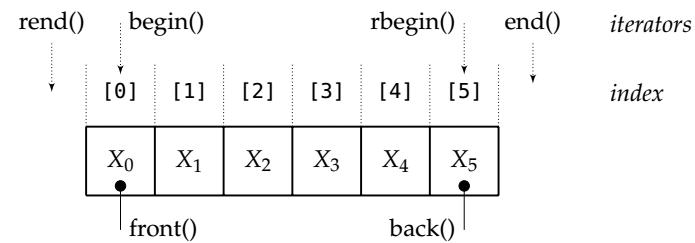
\includegraphics[width=0.7\linewidth]{images/array}
\caption{Array}
\label{fig:array}
\end{figure}
	

\subsection{Vector}
\begin{itemize}
	\item std:vector<T> ist Sequenz von Wert des Types T (Vergleichbar mit einer ArrayList in Java)
	\item Die Elemente des Vectors werden auf dem Heap alloziert (bei Elementen auf dem Stack wird eine Kopie auf den Heap angelegt).
	\item Wird ein Vector einer Funktion übergeben, kann man mit dem Keyword \lstinline|const| verhindern, dass eine Kopie eines sehr grossen Vectors angelegt wird. Wird vom Vector nur gelesen, muss dies in jedem Fall gemacht werden!
	\item Wird der Vector mit runden Klammern initialisiert, alloziert der Compiler die übergeben Anzahl an Elemente. Wenn es geschweifte Klammern sind, wird einfach ein Element mit dem übergebenen Wert übergeben.
\end{itemize}
\begin{lstlisting}[language=C++]
template<class T, class Allocator = std::allocator<T>> class vector;

#include <vector>
#include <algorithm>
#include <iostream>
#include <iterator>

// declaration
std::vector<int> v{1,2,3,4,5} // initialize with 5 elements
std::vector<int> v(6); // alocate 6 elements
std::vector<int> v(6, -1); // allocate with default value
std::vector<std::string> v(6, "hello"); // allocate with default value

// 2d matrix
std::vector<std::vector<std::string>> const matrix { {}, {}, {} };
matrix[i][j];

// add element
v.push_back(val); // add at the tail
v.insert(end(v), val); // add at the tail
v.insert(begin(v), val); // add at the front

// remove elements (1,2,3,4,5)
v.pop_back(); // 1,2,3,4
v.erase(begin(v)); // 2,3,4
v.erase(end(v) + 1, v.end()); // 2
v.clear(); //

// removes the element, but keeps space in vector. (undefined value) erase does also decrease vector size.
remove(begin(v), end(v), element); 

// Find
auto found = find(begin(v), end(v), 42);
if (found != end(v)) {
	out << *found;
}

// Loop
void outputIndex(std::ostream & out, std::vector<int> const & v) {
	for (auto const i: v) {
		out << i << ", ";
	}
	out << "\n";
}

for(auto &e:v) {
	e *= 2; // change element
}

// create vector from stream
using input = std::istream_iterator<int>;
input eof{};
std::vector<int> const v{input{std::cin}, eof};

// fill with input
std::vector<int> v2{};
std::copy(input{std::cin}, eof, back_inserter{v}); // uses push_back

// fill vector
std::vector<int> v(size,default_value); 
// or
std::vector<int> v(10); fill(begin(v), end(v), default_value);

// fill with computed values (1,2,3,4,5...100)
std::vector<int> v(100);
iota(begin(v),end(v), 1);
\end{lstlisting}
\subsubsection{Memberfunktionen}
\begin{description}
	\item[front()] Zugriff auf das erste Element
	\item[back()] Zugriff auf das letzte Element
	\item[insert(index, element)] Einfügen an einer bestimmten Stelle
	\item[at(index)] Element beim Index (Out of Bound Check im Gegensatz zu v[index])
	\item[size()] Länge des Vectors (Variable vom Typ \lstinline|size_t|)
\end{description}
			
\subsection{Double-linked List}
Die Double-linked List erlaubt effizientes einfügen 
Es gibt auch noch eine Singly-linked List. Diesen sollte man aber nicht verwenden. 
\begin{lstlisting}[language=C++]
std::list<> l(<x-times>, <value>)
\end{lstlisting}

\begin{figure}[h]
\centering
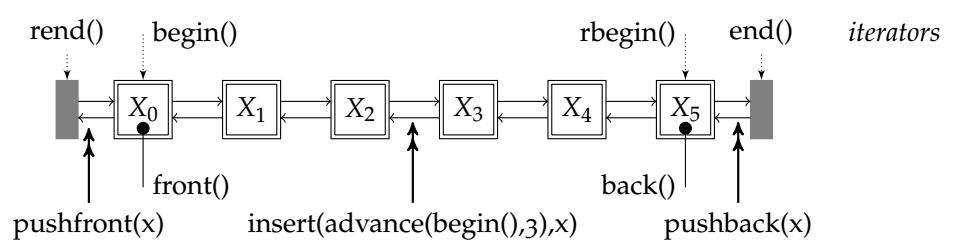
\includegraphics[width=0.5\linewidth]{images/double_linked_list}
\caption{Double-linked List}
\label{fig:doublelinkedlist}
\end{figure}

\subsection{Double-ended Queue, Deque}
Ist wie ein Vector, Objekte können aber zusätzlich effizient am Anfang der Queue eingefügt und entfernt werden. 
\begin{lstlisting}[language=C++]
std::deque<int> q{begin(v),end(v)};
q.pop_front();
q.push_front(42);
q.push_back(42);
q.pop_back();
\end{lstlisting}

\begin{figure}[h]
\centering
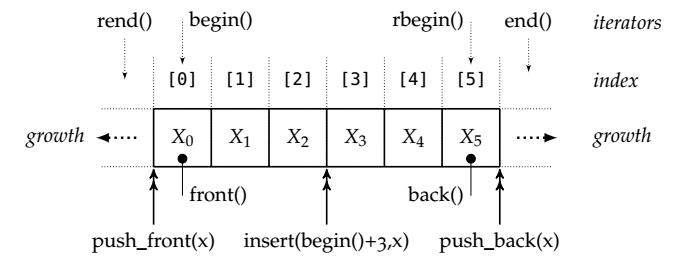
\includegraphics[width=0.5\linewidth]{images/deque}
\caption{Double-ended Queue}
\label{fig:deque}
\end{figure}

\subsection{Queue, FIFO Adapter}
Im Gegensatz zum Stack nimmt \lstinline[]|pop()| die Element am Anfang der Queue raus.
\begin{lstlisting}[language=C++]
std::queue<int> q{};
q.push(42); std::cout << q.front(); q.pop();
\end{lstlisting}
\begin{figure}[h]
\centering
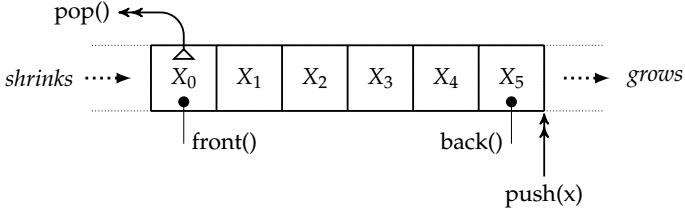
\includegraphics[width=0.5\linewidth]{images/fifo_queue}
\caption{FIFO queue}
\label{fig:fifoqueue}
\end{figure}

\clearpage

\subsection{Stack, LIFO Adapter}			
\begin{lstlisting}[language=C++]
std::stack<int> s{};
s.push(42); std::cout << s.top(); s.pop();
\end{lstlisting}
\begin{figure}[h]
	\centering
	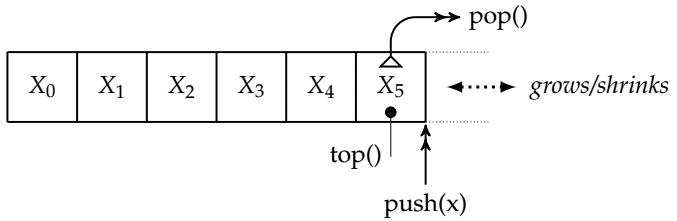
\includegraphics[width=0.5\linewidth]{images/stack}
	\caption{Stack}
	\label{fig:stack}
\end{figure}

\subsection{Set}
Ein Set speichert die Elemente immer sortiert in einem Baum. Es gibt keine Duplikate!
\begin{lstlisting}[language=C++]
std::set<int> s{7,1,4,3,2,5,6};

#include <set>
#include <string>
#include <algorithm> -> transform
#include <iostream> 	-> cout
#include <iterator> 	-> ostream_iterator
#include <cctype> 			-> lowercase

// insert
std::string const input("teststring");
std::set<char> myset { };
std::transform(input.begin(), input.end(), inserter(myset, myset.begin()), 
	[](char c) {
		return tolower(c);
	});

// print
std::ostream_iterator<char> out{std::cout};
std::copy(myset.begin(), myset.end(), out);
\end{lstlisting}

\subsection{Multiset}
Ein Multiset erlaubt Duplikate
\begin{lstlisting}[language=C++]
#include <iostream>
#include <iterator>
#include <string>
#include <set>

using in=std::istream_iterator<std::string>;
using out=std::ostream_iterator<std::string>;
std::multiset<std::string> words{in{std::cin},in{}};
copy(cbegin(words), cend(words), out(std::cout, "\n"));
\end{lstlisting}

\subsection{Map}
Wie beim Set werden die Key-Value paare sortiert gespeichert.
\begin{lstlisting}[language=C++]
std::map<char, size_t> vowels
{{'a',0},{'e',0},{'i',0},{'o',0},{'u',0},{'y',0}};

// Increment Value of Key
++vowels['a'];

// Beim Iterieren ist jedes Element ein pair<char, size>
for(auto const &p:vowels) { 
	std::cout << p.first << " = "<< p.second << '\n';
}
\end{lstlisting}
\begin{figure}[h]
\centering
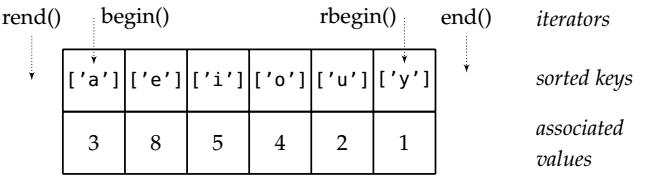
\includegraphics[width=0.5\linewidth]{images/map}
\caption{Map}
\label{fig:map}
\end{figure}

\newpage
\subsection{Multimap}
Die Multimap erlaubt mehrere Keys

\subsection{Hash Container}
In C++ muss man sich selber um die Hashfunktion \lstinline[]|std::hash<>| kümmern. Die Hashcontainer sind nie sortiert. Es gibt zwei Hash Container:

\begin{itemize}
	\item Unordered Set
	\item Unordered Map
\end{itemize}


\section{Iteratoren}
Man hat immer zwei Iteratoren (begin() und end()). Man kann auch die Liste von hinten nach vorne durchlaufen (rbegin() und rend()). Werden die Member nur gelesen werden müssen, können auch das \lstinline|const| Pendant cbegin(), cend(), crbegin() und crend() verwendet werden.

\begin{lstlisting}[language=C++]
// Read only use: use cbegin() und cend()
for (auto it=begin(v); it!=end(v); ++it) {
	// access current element with (*element)
	std::cout << (*it)++ << ", ";
}
\end{lstlisting}

\begin{figure}[h!]
	\centering
	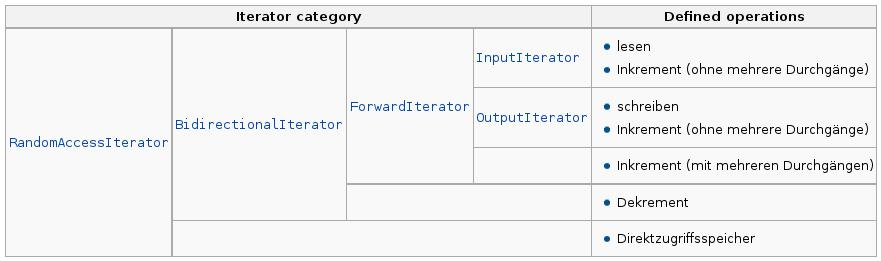
\includegraphics[width=0.9\linewidth]{images/iterator_overview}
	\caption{Iterator Übersicht}
	\label{fig:iteratoroverview}
\end{figure}


\subsection{Algorithmen}
\begin{itemize}
	\item \lstinline|std::advance(iter, n)| überspringt n Iterationen in einem Sprung
	\item \lstinline|std::next(iter, n)| macht das Selbe wie advance(), verändert aber den Iter Parameter nicht. (\lstinline|*next(begin(c), 2)|)
	\item \lstinline|std::distance(from, to)| Zählt die Anzahl Element in dem Bereich
\end{itemize}

\subsection{Typen}
Es gibt 5 verschiedene Iterator Typen:
\begin{lstlisting}[language=C++]
struct input_iterator_tag { };
struct output_iterator_tag { };
struct forward_iterator_tag : public input_iterator_tag { };
struct bidirectional_iterator_tag : public forward_iterator_tag { };
struct random_access_iterator_tag : public bidirectional_iterator_tag { };
\end{lstlisting}

\clearpage

\subsection{Input Iterator}
\begin{itemize}
	\item Aktuelles Element kann genau einmal gelesen werden, danach muss der Iterator inkrementiert werden.(Ganze Sequenz kann also genau einmal durchlaufen werden)
	\item Verwendet für \lstinline|std::istream_iterator| and \lstinline|std::istreambuf_iterator|
\end{itemize}
\begin{lstlisting}[language=C++]
struct input_iterator_tag { };
T const operator *()
operator++()
operator++(int)
operator==(myiter) // and !=
\end{lstlisting}

\subsection{Forward Iterator}
\begin{itemize}
	\item Aktuelles Element kann gelesen und verändert werden (ausser Element oder Container ist const)
	\item Erlaubt nur vorwärts Iteration
	\item Sequenz kann mehrfach durchlaufen werden
\end{itemize}
\begin{lstlisting}[language=C++]
struct forward_iterator_tag { };
T & operator *() const
operator++()
operator++(int)
operator==(myiter) // and !=
\end{lstlisting}


\subsection{Bidirectional Iterator}
\begin{itemize}
	\item Aktuelles Element kann gelesen und verändert werden (ausser Element oder Container ist const)
	\item Erlaubt Iteration vorwärts und rückwärts
	\item Sequenz kann mehrfach durchlaufen werden
	\item Der Random Acccess Iterator verhält sich gleich wie der Bidirectional Iterator, mit dem Unterschied, dass er den Zugriff mit Index [] erlaubt.
\end{itemize}
\begin{lstlisting}[language=C++]
struct bidirectional_iterator_tag { };
T & operator *() const
operator++()
operator++(int)
operator--()
operator--(int)
operator==(myiter)
operator!=(myiter)
\end{lstlisting}

\subsection{Output Iterator}
\begin{itemize}
	\item Aktuelles Element kann einmal verändert werden, danach muss der Iterator inkrementiert werden
	\item Es gibt kein definiertes Ende für die Sequenz (Beispiel: Konsole)
	\item Verwendet für \lstinline|std::ostream_iterator|
	\item Schreibt das Resultat ohne über das Ende bescheid zu wissen
\end{itemize}
\begin{lstlisting}[language=C++]
 struct output_iterator_tag { };
 T& operator *()
 operator++()
 operator++(int)
\end{lstlisting}

\begin{figure}[h]
	\centering
	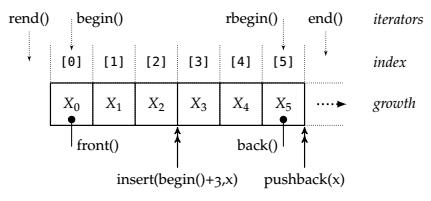
\includegraphics[width=0.7\linewidth]{images/iterator}
	\caption{Iteratoren}
	\label{fig:iterator}
\end{figure}

\subsubsection{\lstinline|back_insert_iterator|}
\lstinline|std::back_insert_iterator| ist ein \lstinline|OutputIterator| welches Elemente an den übergebenen Container mit \lstinline|push_back()| anhängt.

Oft wird für den \lstinline|back_insert_iterator| die Hilfsfunktion \lstinline|std::back_inserter| zur Hilfe genommen:

\begin{lstlisting}[language=C++]
using iiw=std::istream_iterator<Word>;

iiw it { lineIs };
std::vector<Word> words { };
std::copy(iiw(it), iiw(), back_inserter(words));

\end{lstlisting}

\clearpage

\subsection{Loops}
Index basierte for-Loops sollte wenn möglich nicht verwendet werden. Erlaubt sind jedoch die folgenden Range Based for-Loops. Diese arbeiten mit den begin() und end() Iteratoren.
\begin{lstlisting}[language=C++]
for (auto const e : v) {
	out << e;
}

for(auto &e:v) {
	e *= 2; // change element
}

for (auto it=v.begin(); it != v.end(); ++it) {
	// same as for(auto e:v)
}
\end{lstlisting}

	
\subsubsection{Algorithmen}
\begin{description}
	\item[for\_each()] Loope über alle Element
	\begin{lstlisting}
	for_each(rbegin(v), rend(v), [&out](auto x){out << x});
	\end{lstlisting}
	\item[count(begin, end, value)] Zähle das vorkommen des Zeichens \lstinline|value|
	\begin{lstlisting}
	int linecount(std::istream &in, char c){
		using it=std::istreambuf_iterator<char>;
		return count(it{in}, it{}, c);
	}
	\end{lstlisting}
	\item[find(begin, end, value)] Such \lstinline|value| in Container\newpage
	\item[copy(begin, end, begin\_target)] Kopiere Inhalt eines Containers in einen anderen
	\begin{lstlisting}
	// fill vector with content
	std::vector<int> v{};
	using intiter = std::istream_iterator<int>;
	copy(intiter{in}, intiter{}, back_inserter(v));
	return v;
	
	// is equal to the directly method
	std::vector<int> fill(std::istream &in) {
		using intiter = std::istream_iterator<int>;
		return std::vector<int>{intiter{in}, intiter{}};
	}
	\end{lstlisting}
	\item[accumulate(begin, end, startValue)] Summere auf, beginnend bei \lstinline|startValue|
	\item[distance(begin, end)] Anzahl Elemente im Range
	\begin{lstlisting}
	int charCount(std::istream &in) {
		using it = std::istream_iterator<char>; //Excl whitespaces
		using it = std::istreambuf_iterator<char>; // Incl whitespaces
		// begin() = input iterator, end()= empty iterator, not bound to any stream
		return distance(it { in }, it { });
	}
	\end{lstlisting}
	\item[advance(it, n)] Verschiebt einen Iterator um n Stellen
\end{description}


\subsection{Advance}
\begin{itemize}
	\item modifies its argument
	\item returns nothing
	\item works on input iterators or better (or bi-directional iterators if a negative distance is given)
\end{itemize}

\subsection{Next}
\begin{itemize}
	\item leaves its argument unmodified
	\item returns a copy of the argument, advanced by the specified amount
	\item works on forward iterators or better (or bi-directional iterators if a negative distance is given)
\end{itemize}


\newpage
\subsection{Spezielle Iteratoren}
\begin{lstlisting}[language=C++]
std::ostream_iterator<T>
std::istream_iterator<T>

// Alles kommagetrennt ausgeben (std::cout nur in main benutzen! sonst untestbar)
copy(begin(v), end(v), std::ostream_iterator<int>{std::cout, ", "});

// Whitespace werden nicht uebersprungen
std::istreambuf_iterator<char>;
std::ostreambuf_iterator<char>;

// does not skip whitespaces (use get())
using input=std::istreambuf_iterator<char>;
input eof{};
input in{std::cin};
std::ostream_iterator<char> out{std::cout};
copy(in,eof,out);
\end{lstlisting}

\section{STL Algorithmen}
Algorithmen bieten drei klare Vorteile gegenüber handgeschriebene loops:
\begin{enumerate}
	\item Weniger Fehleranfällig
	\item Lesbarer
	\item Je nach Implementierung schneller
\end{enumerate}
\begin{lstlisting}[language=C++, caption=Algorithmen Headers]
// filling, finding, checks, transformation
#include <algorithm>

// accumulate, inner_product, partial_sum, adjacent_difference, iota
#include <numeric> 
\end{lstlisting}

\begin{figure}[h]
\centering
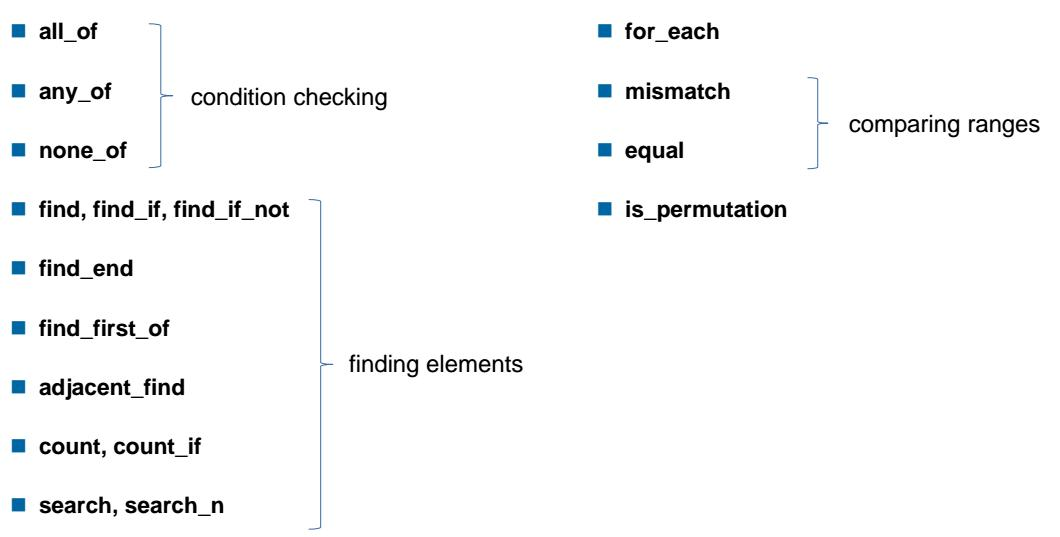
\includegraphics[width=0.7\linewidth]{images/non_modifying_algorithms}
\caption{Nicht verändernde Algorithmen}
\label{fig:nonmodifyingalgorithms}
\end{figure}

\begin{figure}[h]
\centering
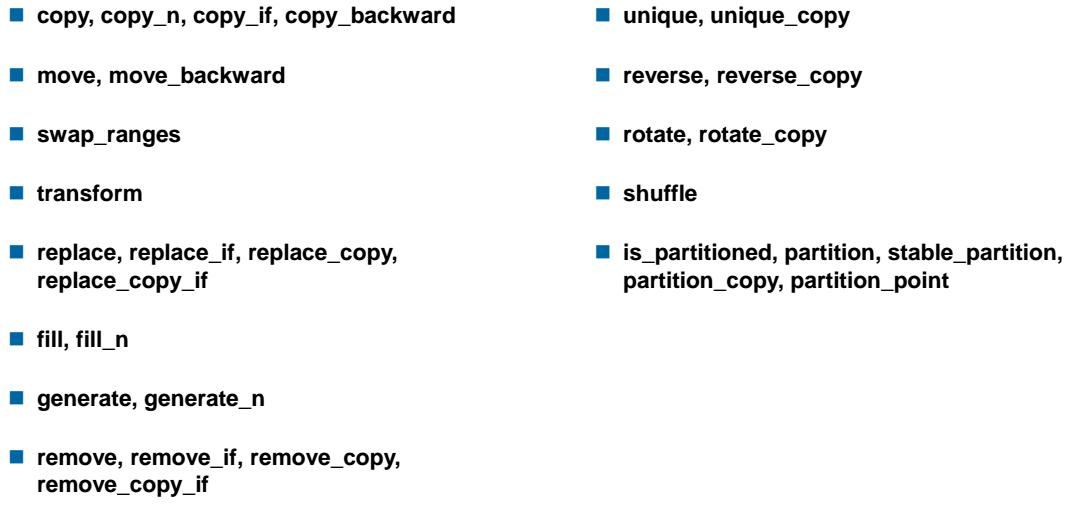
\includegraphics[width=0.7\linewidth]{images/mutating_algorithms}
\caption{Verändernde Algorihtmen}
\label{fig:mutatingalgorithms}
\end{figure}

\begin{figure}[h]
\centering
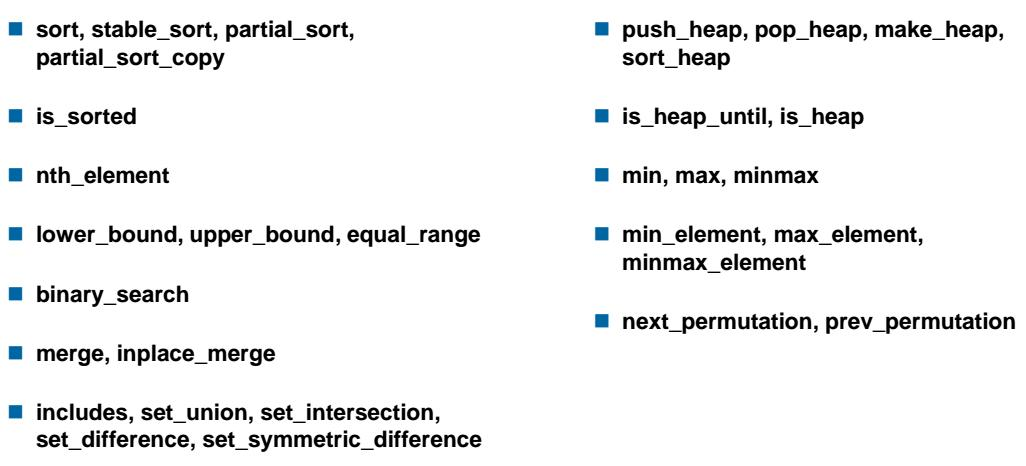
\includegraphics[width=0.7\linewidth]{images/sorting_algorithms}
\caption{Sortierende Algorithmen}
\label{fig:sortingalgorithms}
\end{figure}

\subsection{Min und Max Element Algorithm}
\begin{lstlisting}[language=C++, caption=Max Element Algorithm]
// expected = 1;
auto res = std::min({9, 6, 5, 1, 2, 10, 3, 8});

// expected = 10
auto res = std::max({9, 6, 5, 1, 2, 10, 3, 8});

// expected pair[1,10]
auto res = std::minmax({9, 6, 5, 1, 2, 10, 3, 8});

// expected begin(in1) + 3
std::vector<int> in1{9, 6, 5, 1, 2, 10, 3, 8};
auto res = std::min_element(std::begin(in1), std::end(in1));

// expected begin(in1) + 5 
std::vector<int> in1{9, 6, 5, 1, 2, 10, 3, 8};
auto res = std::max_element(std::begin(in1), std::end(in1));

// expected begin(in1) + 3 , begin(in1) + 5
std::vector<int> in1{9, 6, 5, 1, 2, 10, 3, 8};
auto res = std::minmax_element(std::begin(in1), std::end(in1));
\end{lstlisting}

\subsection{Checking Algorithm}
\begin{lstlisting}[language=C++, caption=Property Checking Algorithm]
// Checks that a predicate is false for at least an element of a sequence
std::vector<unsigned> in1{2, 3, 5, 6, 7};
bool res = std::any_of(
	std::begin(in1),
	std::end(in1),
	is_prime);

// expected true: Checks whether a permutation of the second sequence is equal to the first sequence
std::vector<int> in1{1, 2, 3, 4, 5, 6, 7, 8};
std::vector<int> in2{1, 5, 7, 4, 2, 6, 3, 8};
auto res = std::is_permutation(
	std::begin(in1),
	std::end(in1),
	std::begin(in2));

// expected = std::make_pair(std::begin(in1) + 4, std::begin(in2) + 4);	
std::vector<int> in1{1, 2, 3, 4, 5, 6, 7, 8};
std::vector<int> in2{1, 2, 3, 4, 0, 6, 7, 8};
auto res = std::mismatch(
	std::begin(in1),
	std::end(in1),
	std::begin(in2));
	
// Checks that a predicate is true for all the elements of a sequence
std::vector<unsigned> in1{2, 3, 5, 6, 7};
bool res = std::all_of(
	std::begin(in1),
	std::end(in1),
	is_prime);
	
// auto expected = false;
std::vector<int> in1{1, 2, 3, 4, 5, 6, 7, 8};
std::vector<int> in2{1, 2, 3, 4, 0, 6, 7, 8};
auto res = std::equal(
	std::begin(in1),
	std::end(in1),
	std::begin(in2));
	
// expected true
std::vector<unsigned> in1{1, 4, 6, 8, 9};
bool res = std::none_of(
	std::begin(in1),
	std::end(in1),
	is_prime);
\end{lstlisting}

\subsection{Find Algorithm}
\begin{lstlisting}[language=C++, caption=Find Algorithm]
find(begin(values), end(values), sought) != end(values));

// Find the first occurrence of a value in a sequence
// expected = std::begin(in1) + 4
std::vector<int> in1{1, 2, 3, 4, 5, 6, 7};
auto res = std::find(
	std::begin(in1),
	std::end(in1),
	5);
	
// std::find_if
auto res = std::find_if(
	std::begin(in1),
	std::end(in1),
	is_prime);
	
// Find two adjacent values in a sequence that are equal. 
std::vector<int> in1{5, 6, 4, 7, 7, 2, 2};
auto res = std::adjacent_find(
	std::begin(in1),
	std::end(in1));

// Find element from a set in a sequence
// expected = std::begin(in1) + 5;
std::vector<int> in1{5, 6, 4, 7, 6, 2, 1};
std::vector<int> in2{1, 2, 3};
auto res = std::find_first_of(
	std::begin(in1),
	std::end(in1),
	std::begin(in2),
	std::end(in2));

// Find the first element in a sequence for which a predicate is true
// expected = std::begin(in1) + 1;
std::vector<int> in1{1, 2, 3, 4, 5, 6, 7};
auto res = std::find_if(
	std::begin(in1),
	std::end(in1),
	is_prime);
	
// Find two adjacent values in a sequence that are equal
// expected = std::begin(in1) + 3;
std::vector<int> in1{5, 6, 4, 7, 7, 2, 2};
auto res = std::adjacent_find(
	std::begin(in1),
	std::end(in1));

// Find the first element in a sequence for which a predicate is false
// expected = std::end(in1);
std::vector<int> in1{2, 3, 5, 7, 11, 13, 17};
auto res = std::find_if_not(
	std::begin(in1),
	std::end(in1),
	is_prime);

// Find last matching subsequence in a sequence
// expected = std::begin(in1) + 3;	
std::vector<int> in1{1, 2, 3, 1, 2, 3, 1};
std::vector<int> in2{1, 2, 3};
auto res = std::find_end (
	std::begin(in1),
	std::end(in1),
	std::begin(in2),
	std::end(in2));
\end{lstlisting}

\subsection{Search Algorithm}
\begin{lstlisting}[language=C++, caption=Seach Algorithm]
// Search a sequence for a matching sub-sequence
// expected = std::begin(in1) + 4;
std::vector<int> in1{1, 2, 1, 2, 1, 2, 3, 1, 2, 3};
std::vector<int> in2{1, 2, 3};
auto res = std::search(
	std::begin(in1),
	std::end(in1),
	std::begin(in2),
	std::end(in2));
	
// Search a sequence for a number of consecutive values
// expected = std::begin(in1) + 5;
std::vector<int> in1{1, 1, 2, 2, 2, 1, 1, 1, 3, 3};
	auto res = std::search_n(
	std::begin(in1),
	std::end(in1),
	3,
	1);
\end{lstlisting}

\subsection{Sort Algorithm}
\begin{lstlisting}
// Sort the elements of a sequence
// expected{1, 2, 3, 4, 5, 6, 7, 8, 9}
std::vector<int> in_out1{2, 3, 5, 7, 1, 4, 6, 8, 9};
std::sort(
	std::begin(in_out1),
	std::end(in_out1));


// Copy the smallest elements of a sequence
// expected{1, 2, 3, 4, 5}
std::vector<int> in1{2, 5, 3, 7, 1, 4, 6, 8, 9};
std::vector<int> out1{0, 0, 0, 0, 0};
std::partial_sort_copy(
	std::begin(in1),
	std::end(in1),
	std::begin(out1),
	std::end(out1));

// Determines whether the elements of a sequence are sorted
std::vector<unsigned> in1{2, 3, 5, 6, 7};
bool res = std::is_sorted(
	std::begin(in1),
	std::end(in1));

// Sort the smallest elements of a sequence
// expected{1, 2, 3, 4}
std::vector<int> in_out1{2, 5, 3, 7, 1, 4, 6, 8, 9};
std::partial_sort(
	std::begin(in_out1),
	std::begin(in_out1) + 4,
	std::end(in_out1));

// Sort the elements of a sequence using a predicate for comparison, preserving the relative order of equivalent elements
// std::vector<std::pair<int, int>> expected{{1, 0}, {1, 2}, {1, 4}, {2, 1}, {2, 3}};
std::vector<std::pair<int, int>> in_out1{{2, 1}, {1, 0}, {1, 2}, {1, 4}, {2, 3}};
std::stable_sort(
	std::begin(in_out1),
	std::end(in_out1),
	[](std::pair<int, int> l, std::pair<int, int> r) {return l.first < r.first;});

// Sort a sequence just enough to find a particular position
std::vector<unsigned> in_out1{45, 27, 73, 15, 95, 64, 44, 0, 99};
std::nth_element(
	std::begin(in_out1),
	std::begin(in_out1) + 3,
	std::end(in_out1));
\end{lstlisting}
\newpage

\subsection{Sorted Sequence Algorithms}
\begin{lstlisting}
// Merges two sorted ranges in place
// expected{1, 2, 3, 3, 7, 8, 9, 10, 13, 15, 16}
std::vector<int> in_out1{2, 3, 8, 9, 10, 16, 1, 3, 7, 13, 15};
std::vector<int> ;
	std::inplace_merge(
	std::begin(in_out1),
	std::begin(in_out1) + 6,
	std::end(in_out1));

// Determines whether an element exists in a range
std::vector<int> in1{1, 2, 3, 4, 5, 6, 7, 8, 9};
auto res = std::binary_search(
	std::begin(in1),
	std::end(in1),
	7);

// Merges two sorted ranges
// expected{1, 2, 3, 3, 7, 8, 9, 10, 13, 15, 16};
std::vector<int> in1{1, 3, 7, 13, 15};
std::vector<int> in2{2, 3, 8, 9, 10, 16};
std::vector<int> out{};
std::merge(
	std::begin(in1),
	std::end(in1),
	std::begin(in2),
	std::end(in2),
	std::back_inserter(out));


// Finds the largest subrange in which val could be inserted at any place in it without changing the ordering
// auto expected = std::make_pair(std::begin(in1) + 3, std::begin(in1) + 6);
std::vector<unsigned> in1{1, 1, 1, 2, 2, 2, 3, 4, 4};
auto res = std::equal_range(
	std::begin(in1),
	std::end(in1),
	2);

// Finds the first position in which @a val could be inserted without changing the ordering	
std::vector<unsigned> in1{1, 1, 1, 2, 2, 2, 3, 4, 4};
auto expected = std::begin(in1) + 3;
	auto res = std::lower_bound(
	std::begin(in1),
	std::end(in1),
	2);
\end{lstlisting}

\subsection{Count Algorithm}
\begin{lstlisting}[language=C++, caption=Count Algorithm]
// Count the number of copies of a value in a sequence
// expected 4 matches
std::vector<int> in1{1, 2, 3, 2, 1, 2, 3, 4, 3, 2};
int res = std::count(
	std::begin(in1),
	std::end(in1),
	2);

// Count the elements of a sequence for which a predicate is true
// int expected = 4;
std::vector<int> in1{1, 2, 3, 4, 5, 6, 7, 8, 9, 10};
int res = std::count_if(
	std::begin(in1),
	std::end(in1),
	is_prime);
\end{lstlisting}

\subsection{Set Algorithm}
\begin{lstlisting}[language=C++, caption=Set Algorithm]
// Return the intersection of two sorted ranges
// expected{4, 5, 6, 9}
std::vector<int> in1{1, 2, 3, 4, 5, 6, 7, 8, 9};
std::vector<int> in2{4, 5, 6, 9, 10, 11, 12};
std::vector<int> out{};

std::set_intersection(
	std::begin(in1),
	std::end(in1),
	std::begin(in2),
	std::end(in2),
	std::back_inserter(out));
	
// Return the difference of two sorted ranges
// expected{1, 2, 3, 7, 8}
std::vector<int> in1{1, 2, 3, 4, 5, 6, 7, 8, 9};
std::vector<int> in2{4, 5, 6, 9, 10, 11, 12};
std::vector<int> out{};

std::set_difference(
	std::begin(in1),
	std::end(in1),
	std::begin(in2),
	std::end(in2),
	std::back_inserter(out));
	
// Return the union of two sorted ranges
// expected{1, 2, 3, 4, 5, 6, 7, 8, 9, 10, 11, 12};
std::vector<int> in1{1, 2, 3, 4, 5, 6, 7, 8, 9};
std::vector<int> in2{4, 5, 6, 9, 10, 11, 12};
std::vector<int> out{};
std::vector<int> 

std::set_union(
	std::begin(in1),
	std::end(in1),
	std::begin(in2),
	std::end(in2),
	std::back_inserter(out));
	
// Return the symmetric difference of two sorted ranges
// expected{1, 2, 3, 7, 8, 10, 11, 12}
std::vector<int> in1{1, 2, 3, 4, 5, 6, 7, 8, 9};
std::vector<int> in2{4, 5, 6, 9, 10, 11, 12};
std::vector<int> out{};
std::set_symmetric_difference(
	std::begin(in1),
	std::end(in1),
	std::begin(in2),
	std::end(in2),
	std::back_inserter(out));
	
// Determines whether all elements of a sequence exists in a range
std::vector<int> in1{1, 2, 3, 4, 5, 6, 7, 8, 9};
std::vector<int> in2{2, 3, 4, 7, 8, 9};
auto res = std::includes(
	std::begin(in1),
	std::end(in1),
	std::begin(in2),
	std::end(in2));
\end{lstlisting}

\subsection{Copy Algorithm}
\begin{lstlisting}[language=C++, caption=Copy Algorithm]
// Leite den kompletten Input in den Output
using in_iter = std::istream_iterator<char>;
using out_iter = std::ostream_iterator<char>;
std::copy(in_iter{in}, in_iter{}, out_iter{out});

// expected {5, 6, 3, 5, 6, 3, 7, 4};
std::vector<int> in_out1{5, 6, 3, 7, 4, 0, 0, 0};
std::copy_backward(
	std::begin(in_out1),
	std::begin(in_out1) + 5,
	std::end(in_out1));

// expected {5, 6, 3, 7, 9, 1, 5};
std::vector<int> in1{5, 6, 3, 7, 9, 1, 5};
std::vector<int> out1{};
std::copy(
	std::begin(in1),
	std::end(in1),
	std::back_inserter(out1));
	
// expected {5, 3, 7, 5};
std::vector<int> in1{5, 6, 3, 7, 10, 10, 5};
std::vector<int> out1{};
std::copy_if(
	std::begin(in1),
	std::end(in1),
	std::back_inserter(out1),
	[](int const & i) {return i % 2;});

// expected {5, 6, 3, 7, 9, 1};
std::vector<int> in1{5, 6, 3, 7, 9, 1, 5};
std::vector<int> out1{}; 
std::copy_n(
	std::begin(in1),
	6,
	std::back_inserter(out1));
\end{lstlisting}


\subsection{Replace Algorithm}
\begin{lstlisting}[language=C++, caption=Replace Algorithm]
// 1, 4, 3, 4, 1, 4, 3, 4
std::vector<int> in_out1{1, 2, 3, 2, 1, 2, 3, 2};
std::replace(
	std::begin(in_out1),
	std::end(in_out1),
	2,
	4);
	
// std::replace_if: expected{1, 0, 0, 4, 0, 6, 0, 8};
std::replace_if(
	std::begin(in_out1),
	std::end(in_out1),
	is_prime,
	0);

//	std::replace_copy_if: expected{5, 6, 3, 7, 9, 1};
std::vector<int> out1{};
std::replace_copy_if(
	std::begin(in1),
	std::end(in1),
	std::back_inserter(out1),
	is_prime,
	0);
\end{lstlisting}


\subsection{Transform Algorithm}
\begin{lstlisting}[language=C++, caption=Transform Algorithm]
// Transform: Print a letter x Times, according to counts
std::vector<int> counts{3, 0, 1, 4, 0, 2};
std::vector<char> letters{'g', 'a', 'u', 'y', 'f', 'o'};
std::vector<std::string> combined{};
auto times = [](int i, char c) {return std::string(i, c);};
std::transform(begin(counts), end(counts), begin(letters), 
	std::back_inserter(combined), times);

// 2^x: expected 32, 64, 128, 256, 1, 1024
std::vector<int> in1{5, 6, 7, 8, 0, 10};
std::vector<int> out1{};

std::transform(
		std::begin(in1),
		std::end(in1),
		std::back_inserter(out1),
		[](int i){return std::pow(2, i);});
\end{lstlisting}

\newpage
\subsection{Swap Algorithm}
\begin{lstlisting}[language=C++, caption=Transform Algorithm]
// Swapt die beiden Vector in den jeweilig anderen
std::vector<int> in_out1{1, 2, 3, 4};
std::vector<int> in_out2{5, 6, 7, 8};

std::swap_ranges(
	std::begin(in_out1),
	std::end(in_out1),
	std::begin(in_out2));
\end{lstlisting}

\subsection{Merge Algorithm}
\begin{lstlisting}[language=C++, caption=Merge Algorithm]
// Merge two sorted ranges
std::vector<int> r1{9, 12, 17, 23, 54, 57, 85, 95};
std::vector<int> r2{2, 30, 32, 41, 49, 63, 72, 88};
std::vector<int> d(r1.size() + r2.size(), 0);
std::merge(begin(r1), end(r1), begin(r2), end(r2), begin(d));
\end{lstlisting}

\subsection{Erase-Remove-Idiom}
Das \lstinline|remove_if| verschiebt die validen Element einfach nach vorne und überschreibt damit die invaliden Elemente. Am Ende des Vectors bleiben dann Elemente mit unbekanntem Status übrig. Diese können mit dem Algorithmus \lstinline|remove| entfernt werden.
\begin{lstlisting}[language=C++, caption=Erase-Remove-Idiom]
//  Transforms the range [first,last) into a range with all the elements for which pred returns true removed, and returns an iterator to the new end of that range.
std::vector<unsigned> values{54, 13, 17, 95, 2, 57, 12, 9};
auto is_prime = [](unsigned u) {/*...*/};
auto removed = std::remove_if(begin(values), end(values), is_prime);
values.erase(removed, values.end()); // actually remove items


// expected{1, 3, 1, 3}: Remove elements from a sequence
std::vector<int> in_out1{1, 2, 3, 2, 1, 2, 3, 2};
auto new_end = std::remove(
	std::begin(in_out1),
	std::end(in_out1),
	2);
	
// expected{1, 4, 6, 8};
std::vector<int> in_out1{1, 2, 3, 4, 5, 6, 7, 8};
auto new_end = std::remove_if(
	std::begin(in_out1),
	std::end(in_out1),
	is_prime);
	
// expected{1, 4, 6, 8}
std::vector<int> in1{1, 2, 3, 4, 5, 6, 7, 8};
std::vector<int> out1{};
std::remove_copy_if(
	std::begin(in1),
	std::end(in1),
	std::back_inserter(out1),
	is_prime);
	
// expected{1, 3, 1, 3}
std::vector<int> in1{1, 2, 3, 2, 1, 2, 3, 2};
std::vector<int> out1{};
std::remove_copy(
	std::begin(in1),
	std::end(in1),
	std::back_inserter(out1),
	2);
\end{lstlisting}

\subsection{Reverse Algorithm}
\begin{lstlisting}[language=C++, caption=Reverse Algorithm]
// Dreht einen std::vector<int> & values
reverse(begin(values), end(values));

// Copy a sequence, reversing its elements
// expected{10, 0, 8, 7, 6, 5}
std::vector<int> in1{5, 6, 7, 8, 0, 10};
std::vector<int> out1{};
std::reverse_copy(
	std::begin(in1),
	std::end(in1),
	std::back_inserter(out1));

// expected{10, 0, 8, 7, 6, 5}: Reverse a sequence
std::vector<int> in_out1{5, 6, 7, 8, 0, 10};
std::reverse(
	std::begin(in_out1),
	std::end(in_out1));
\end{lstlisting}


\subsection{Unique Algorithmen}
\begin{lstlisting}[language=C++, caption=Unique Algorithmen]
// Remove consecutive duplicate values from a sequence
// expected{1, 3, 4, 2}
std::vector<int> in_out1{1, 1, 3, 3, 4, 2, 2, 2};

auto new_end = std::unique(
	std::begin(in_out1),
	std::end(in_out1));

// Copy a sequence, removing consecutive duplicate values
// expected{1, 3, 4, 2};
std::vector<int> in1{1, 1, 3, 3, 4, 2, 2, 2};
std::vector<int> out1{};

std::unique_copy(
	std::begin(in1),
	std::end(in1),
	std::back_inserter(out1));
\end{lstlisting}

\subsection{Rotate Algorithm}
\begin{lstlisting}
// Rotate the elements of a sequence
// expected{5, 6, 7, 8, 9, 1, 2, 3, 4}
std::vector<int> in_out1{1, 2, 3, 4, 5, 6, 7, 8, 9};
std::rotate(
	std::begin(in_out1),
	std::begin(in_out1) + 4,
	std::end(in_out1));

// Copy a sequence, rotating its elements
// expected{5, 6, 7, 8, 9, 1, 2, 3, 4}
std::vector<int> in1{1, 2, 3, 4, 5, 6, 7, 8, 9};
std::vector<int> out1{};
std::rotate_copy(
	std::begin(in1),
	std::begin(in1) + 4,
	std::end(in1),
	std::back_inserter(out1));
\end{lstlisting}

\subsection{Numerische Algorithmen}
\begin{lstlisting}
// Create a range of sequentially increasing values
// expceted 0, 1, 2, 3, 4, 5, 6, 7
std::vector<int> out1(8);
std::iota(std::begin(out1), std::end(out1), 0);

// Return differences between adjacent values
// expected 1, 1, 2, -1, 6, -4, 2
std::vector<int> in1{1, 2, 4, 3, 9, 5, 7};
std::vector<int> out1(in1.size());
std::adjacent_difference(std::begin(in1), std::end(in1), 	std::begin(out1));


// expected 121: Accumulate values in a range
std::vector<int> in1{1, 2, 3, 4, 5, 6};
int res = std::accumulate(std::begin(in1), std::end(in1), 100);

// 1, 21,321,4321, 54321: Return list of partial sums
std::vector<int> in1{1, 20, 300, 4000, 50000};
std::vector<int> out1(in1.size());
std::partial_sum(std::begin(in1), std::end(in1), std::begin(out1));

// Compute inner product of two ranges
// "begin, 1a, 2b, 3c, 2d, 1e"
std::vector<int> in1{1, 2, 3, 2, 1};
std::vector<char> in2{'a', 'b', 'c', 'd', 'e'};

std::string res = std::inner_product (
		std::begin(in1),
		std::end(in1),
		std::begin(in2),
		std::string{"begin"},
		[](std::string l, std::string r) {return l + ", " + r;},
		[](int i, char c) {return std::to_string(i) + c;});
\end{lstlisting}

\newpage
\subsection{Partition Algorithmen}
\begin{lstlisting}
// move elements for which a predicate is true to the beginning of a sequence,
// expected{7, 2, 3, 5, 4, 6, 1, 8, 9};
std::vector<int> in_out1{1, 2, 3, 4, 5, 6, 7, 8, 9};
std::partition(
	std::begin(in_out1),
	std::end(in_out1),
	is_prime);
	
// same as partition, but preserving relative ordering.
// expected {2, 3, 5, 7, 1, 4, 6, 8, 9};
std::vector<int> in_out1{1, 2, 3, 4, 5, 6, 7, 8, 9};
std::stable_partition(
	std::begin(in_out1),
	std::end(in_out1),
	is_prime);

// Find the partition point of a partitioned range
// expected = std::begin(in1) + 4;
std::vector<int> in1{2, 3, 5, 7, 1, 4, 6, 8, 9};
auto res = std::partition_point(
	std::begin(in1),
	std::end(in1),
	is_prime);
	
// expected true: Checks whether the sequence is partitioned
std::vector<int> in1{2, 3, 5, 7, 1, 4, 6, 8, 9};
bool res = std::is_partitioned(
	std::begin(in1),
	std::end(in1),
	is_prime);
\end{lstlisting}

\subsection{Accumulate}
Accumulate wird standardmässig fürs aufsummieren verwendet. Man kann ihn aber auch verwenden, wenn z.B ein Komma nur zwischen den Elementen eingefügt werden soll (und nicht am Ende).
\begin{lstlisting}[language=C++, caption=Accumulate]
std::vector<std::string> long_months{"Jan", "Mar", "May", "Jul", "Aug", "Oct", "Dec"};
std::string accumulated_string = std::accumulate(
	begin(long_months) + 1, //Second element
	end(long_months),       //End
	long_months.at(0),      //First element, usually the neutral element
	[](std::string const & acc, std::string const & element) {
		return acc + ", " + element;
	}); //Jan, Mar, May, Jul, Aug, Oct, Dec
\end{lstlisting}

\newpage
\subsection{If Algorithmen}
\begin{lstlisting}[language=C++, caption=If Algorithmen]
std::set<unsigned> numbers{1, 2, 3, 4, 5, 6, 7, 8, 9};
auto is_prime = [](unsigned u) {/*...*/};
auto nOfPrimes = std::count_if(begin(numbers), end(numbers), is_prime);

count_if
find_if
find_if_not
copy_if
remove_if
remove_copy_if
replace_if
replace_copy_if
\end{lstlisting}

\subsection{Fill und Generate Algorithmen}
\begin{lstlisting}[language=C++, caption=Fill und Generate Algorithmen]
// Fills the range [first,last) with copies of value.
// expected{42, 42, 42, 42, 42, 42, 42, 42};
std::vector<int> in_out1{1, 2, 3, 4, 5, 6, 7, 8};
std::fill(
	std::begin(in_out1),
	std::end(in_out1),
	42);

// Fills a range with copies of the same value.
//  expected{42, 42, 42, 42, 5, 6, 7, 8};
std::vector<int> in_out1{1, 2, 3, 4, 5, 6, 7, 8};
std::fill_n(
	std::begin(in_out1),
	4,
	42);

// Assign the result of a function object to each value in a sequence
// expected{100, 101, 102, 103, 104};
std::vector<int> out1(5);
int start = 100;
std::generate(
	std::begin(out1),
	std::end(out1),
	[start]() mutable {return start++;});

// Assign the result of a function object to each value in a sequence
// expected{100, 101, 102, 103, 104};
std::vector<int> out1{};
int start = 100;
std::generate_n(
	std::back_inserter(out1),
	5,
	[start]() mutable {return start++;});
\end{lstlisting}

\newpage
\subsection{Heap Algorithmen}
\begin{lstlisting}[language=C++, caption=Heap Algorithmen]
std::vector<int> v{3,1,4,1,5,9,2,6};

// Construct a heap over a range
// Erstelle Heap (Baum von links her aufgefuellt) aus Vector
make_heap{v.begin(), v.end()};

// Switched Root mit letztem Item und stellt Heap Eigenschaft mit Downheap wieder her
pop_heap(v.begin(), v.end());
v.pop_back(); // entfernt das Element vom Heap

// Fuege Element dem Heap hinzu
v.push_back(8);
push_heap(v.begin(), v.end());

// Sortiere den Heap. Dies ist extrem schnell
sort_heap(v.begin(), v.end());
\end{lstlisting}


\subsection{Distance Algorithm}
\begin{lstlisting}[language=C++, caption=Distance ALgorithm] 
#include "wcount.h"
#include "src/word.h"
#include <istream>
#include <iterator>

unsigned wcount(std::istream& in) {
	return std::distance(std::istream_iterator<Word>(in), std::istream_iterator<Word>());
}

// count only different words
unsigned wdiffcount(std::istream& in) {
	std::vector<Word> wordVector{std::istream_iterator<Word>(in), std::istream_iterator<Word>()};
	std::sort(wordVector.begin(), wordVector.end());
	return std::distance(wordVector.begin(), std::unique(wordVector.begin(), wordVector.end()));
}
\end{lstlisting}

\section{Legacy C Structures}
\subsection{C Arrays}
Wenn ein C Array einer Funktion übergeben wird, wird einzig ein Pointer auf das erste Element des Arrays übergeben. Dies Grösseninformation geht dabei verloren.
\begin{lstlisting}[language=C++] 
int a[5];
sum(a); 

int sum(int a[]) { .. }

// Loesung

// oder std::vector<int> v(5);
// oder std::array<int, 5> sa;
// oder template <size_t n> int sum(int (&a)[n]);

// example 
template<typename T, unsigned N> void printArray(std::ostream &out, T const (&x)[N]) {
	copy(x, x+N, std::ostream_iterator<T>{out, ", "});
}

int a[] = {1,2,3}M
printArray(std::cout, a);
\end{lstlisting}


\subsection{Array Pointer}
Array Pointer sind Random Access Iteratoren und können demnach inkrementiert/dekrementiert werden. Diese sollte aber nie so verwendet werden!
\begin{lstlisting}[language=C++]
++p, *p, p+int, p[int], *(p+int)
\end{lstlisting}

\subsection{Array Initialisierung}
Arrays die direkt Initialisiert werden, nehmen implizit die Dimension anhand der Anzahl Elemente. Wird das Array ohne Elemente Initialisiert, wird das Default Value des Types genommen. Wird es nicht initialisiert, kann undefined behaviour entstehen.
\begin{lstlisting}[language=C++, caption=Initializing an Array] 
int five[5] // might be unitialized
int five[5]{}; // 5 zeros
double m[2][3]{{1,2,3},{4,5,6}};
\end{lstlisting}

\section{Dynamic Heap Memory Managemnt}
Das Heap Memory sollte nur in Spezialfällen selbständig verwaltet werden! Deshalb sollte kein \lstinline|new| verwendet werden. (Alloziert Objekte auf dem Heap). Wenn man es trotzdem macht, ist man auch für das Aufräumen verantworlich. Ansonsten drohen Memory Leaks, DanglingPointers und Double Deletes. (es gibt keine Garbage Collection. Die Garbage Collection kommt bei der schliessenden geschweiften Klammer sofern man die Pointer mit einer der folgenden Funktionen erzeugt wurde.). Möchte man Heap Pointer verwenden sollte man dies immer mit \lstinline|std::unique_ptr<T>| oder \lstinline|std::shared_ptr<T>| verwenden. Das PIMPL (Pointer to Implementation) Idiom versteckt die Implementierung der eigentlichen Klassenmember einer Klasse in der Impl-Klasse.
\begin{itemize}
	\item Delete Pointer muss grundsätzlich nie aufgerufen werden
	\item Unique Pointer: Für unshared Heap Memory (Kann nicht kopiert werden)
	\item Shared Pointer: Für geteiltes Heap Memory (Arbeiten ähnlich wie Java Referenzen. Können kopiert und verschoben werden)
	\item Wenn das letzte shared\_ptr Handle zerstört wird, wird das allozierte Objekt gelöscht.
	\item Shared Pointer haben das Problem von Zyklen. Deshalb gibt es den weak\_ptr um die Zyklen aufzubrechen.
\end{itemize}


\begin{lstlisting}
#include <memory>
#include <string>

// real usage of unique heap pointers
std::unique_ptr<T> factory(int i) {
	return std::make_uniqe<T>(i);
}

// or
std::shared_ptr<A> A_factory() {
return std::make_shared<A>(5, "hi", 'a');
}

// real usage of shared heap pointers
struct A {
	A(int a, std::string b, char c) {}
};

int main() {
	auto an_a = A_factory();
	auto b=an_a; // second pointer to same object
	A c{*b};
	auto another = std::make_shared<A>(c);
}
\end{lstlisting}

\clearpage

\begin{lstlisting}
// person.h
#include <memory>
#include <string>
#include <vector>
#include <iosfwd>

// type forward declaration!
using PersonPtr=std::shared_ptr<class Person>;

class Person {
	std::string name;
	std::vector<PersonPtr> children;
public:
	Person(std::string name):name{name}{}
	void addChild(PersonPtr child){
		children.push_back(child);
	}
	void print(std::ostream &) const;

static PersonPtr makePerson(std::string name){
	return std::make_shared<Person>(name);
}
};


// usage
#include "person.h"
std::string name{"name"};
auto pers = Person::makePerson(name);
\end{lstlisting}

\section{Vererbung}
Vererbung wird immer dann verwendet, wenn man Verhalten wiederverwenden und erweitern möchte. (besser: Adapter verwenden) Vererbung ist deshalb schlecht, weil es eine starke Kopplung zwischen den Klassen erzeugt. 
\begin{itemize}
	\item Vererbung ist standardmässig \lstinline|public| (bei Klassen!). Bei Structs ist die Vererbung implizit \lstinline|public|
	\item Die Konstruktoren werden nicht implizit vererbt
	\item Es wird immer zuerst das Parent Objekt konstruiert und danach die Subklassen
	\item \lstinline|const| wird zur Signatur gezählt
	\item Zuweisungen oder übermitteln von Parameter \lstinline|by value| von abgeleiteten Klassen in Variablen vom Typ der Base Klasse resultieren in \textbf{Object Slicing} \\ $\rightarrow$ Nur Base Class Member Variablen werden behalden. (\lstinline|MyBase base = subVar;|)
\end{itemize}

\begin{lstlisting}
class MyClass : Base {}; // implicit private
struct MyStruct : Base {}; // implicit public
class MyClass : public Base {
	public: 
		// inherit constructor
		using Base::Base;
};

// Initializing base classes (super call)
class DerivedWithCtor : public Base {
	DerivedWithCtor():Base{}{} // default constrcutor
};

// always call base class befor member init
class DerivedWithCtro : public Base {
	DerivedWithCtor(int i, int j) : Base{i}, myLocalVar{j} {}
};

// abstract function (zero)
virtual void foo() const = 0; 
\end{lstlisting}

\subsection{Sichtbarkeiten}
\begin{itemize}
	\item public: Member sind sichbar und nutzbar in den abgeleiteten Klassen (solange in der abgeleiteten Klasse \textbf{kein} Member mit dem gleichen Namen definiert ist ) 
	\item protected: Sind nur in abgeleiten Klassen sichtbar
	\item private: Sind nur in der Base Klasse sichtbar
\end{itemize}

\clearpage

\subsection{Dynamic Binding}
Fürs Dynamic Dispatch ist das Keyword \lstinline|virtual| nötig. (Overhead von VTable) Damit die korrekte Funktion aufgerufen wird, wird in der VTable nachgeschaut.

\begin{lstlisting}
class PolymorphicBase {
	public:
	virtual void doit() { /* something*/ }
};
class Implementor: public PolymorphicBase {
	public:
	void doit() {
		/* something else */
	}
};
\end{lstlisting}

\subsection{Abstrakte Klassen}
Abstrakte Methoden werden auch als ''pure virtual'' bezeichnet.
\begin{lstlisting}
struct AbstractBase {
	// base classes with virtual members require a virtual 
	// destructor if heap allocated without shared_ptr (not recommended)
	virtual ~AbstractBase(){}
	
	// abstract member function (zero -> pure virtual)
	virtual void doitnow() = 0;
};
\end{lstlisting}

\section{CUTE}
\begin{lstlisting}[language=C++, caption=Basic CUTE Test File]
#include "cute.h"
#include "ide_listener.h"
#include "xml_listener.h"
#include "cute_runner.h"
#include "sayhello.h"

void testSayHelloSaysHelloWorld() {
	std:ostringstream out{}; // use default constructor
	sayHello(out);
	ASSERT_EQUAL("Hello, world\nLeftarrow", out.str());
}

void runAllTests(int argc, char const *argv[]) {
	cute::suite s;
	
	// TODO add your test here
	
	s.push_back(CUTE(testSayHelloSaysHelloWorld));
	
	cute::xml_file_opener xmlfile(argc,argv);
	cute:xml_listener<cute::ide_listener<> > lis(xmlfile.out);
	cute::makeRunner(lis,argc,argv)(s, "AllTests");
}

int main(int argc, char const *argv[]){
	runAllTests(argc, argv);
}
\end{lstlisting}

\subsection{Streams}
\begin{lstlisting}[language=C++, caption=Test IO Stream]
void wcount(std::istream &in, std::ostream &out) {
	using it=std::istream_iterator<std::string>;
	int count = distance(it{in}, it{});
	out << count;
}

void test() {
	std::istringstream in{"this is a test"};
	std::ostringstream out{};
	wcount(in, out);
	ASSERT_EQUAL("4", out.str());
}

\end{lstlisting}

\subsection{Asserts}
\begin{description}
	\item[Gleichheit] \lstinline|ASSERT_EQUAL()|
	\item[Exceptions] \lstinline|ASSERT_THROWS(empty_vector.at(0), std::out_of_range)|
	\item[Gleitkommazahlen] \lstinline|ASSERT_EQUAL_DELTA()|
\end{description}


\appendix

% Code Listings
\lstlistoflistings

% List of figures
\listoffigures

% List of tables
\listoftables

% Bibliography
\bibliographystyle{plain} 
\bibliography{literatur}

\end{document}